\documentclass{beamer}
\usepackage[T1]{fontenc}
\usepackage[french]{babel}
\usepackage[utf8]{inputenc}
\usepackage{amsmath}
\usepackage{hyperref}
\usepackage{verbatim}
\usepackage{graphicx}
\usepackage{fancyvrb}

\hypersetup{
  backref=true, %permet d'ajouter des liens dans...
  pagebackref=true,%...les bibliographies
  hyperindex=true, %ajoute des liens dans les index
  colorlinks=true, %colorise les liens
  breaklinks=true, %permet le retour a la ligne dans les liens trop longs
  urlcolor=blue,  %couleur des hyperliens (blue pour la version web)
  linkcolor=blue, %couleur des liens internes (blue pour la version web)
  citecolor=blue, %couleur des citation (green pour la version web)
  bookmarks=true,  %cree des signets pour Acrobat
  bookmarksopen=true, %affiche completement les signets Acrobat
  %%%%%%%%%%%%%%%%% HYPER TITLE %%%%%%%%%%%%%%%%%%%%%%%%%%
  pdfsubject={Transparents} %document sous Acrobat.
}

\usetheme{boxes}
% \definecolor{MonJaune}{HTML}{FFCC00}
% \setbeamercolor{block title}{fg=MonJaune}


\makeatletter
\def\PY@reset{\let\PY@it=\relax \let\PY@bf=\relax%
    \let\PY@ul=\relax \let\PY@tc=\relax%
    \let\PY@bc=\relax \let\PY@ff=\relax}
\def\PY@tok#1{\csname PY@tok@#1\endcsname}
\def\PY@toks#1+{\ifx\relax#1\empty\else%
    \PY@tok{#1}\expandafter\PY@toks\fi}
\def\PY@do#1{\PY@bc{\PY@tc{\PY@ul{%
    \PY@it{\PY@bf{\PY@ff{#1}}}}}}}
\def\PY#1#2{\PY@reset\PY@toks#1+\relax+\PY@do{#2}}

\def\PY@tok@gd{\def\PY@tc##1{\textcolor[rgb]{0.63,0.00,0.00}{##1}}}
\def\PY@tok@gu{\let\PY@bf=\textbf\def\PY@tc##1{\textcolor[rgb]{0.50,0.00,0.50}{##1}}}
\def\PY@tok@gt{\def\PY@tc##1{\textcolor[rgb]{0.00,0.25,0.82}{##1}}}
\def\PY@tok@gs{\let\PY@bf=\textbf}
\def\PY@tok@gr{\def\PY@tc##1{\textcolor[rgb]{1.00,0.00,0.00}{##1}}}
\def\PY@tok@cm{\def\PY@tc##1{\textcolor[rgb]{0.50,0.50,0.50}{##1}}}
\def\PY@tok@vg{\let\PY@bf=\textbf\def\PY@tc##1{\textcolor[rgb]{0.82,0.44,0.00}{##1}}}
\def\PY@tok@m{\let\PY@bf=\textbf\def\PY@tc##1{\textcolor[rgb]{0.38,0.00,0.88}{##1}}}
\def\PY@tok@mh{\let\PY@bf=\textbf\def\PY@tc##1{\textcolor[rgb]{0.00,0.31,0.50}{##1}}}
\def\PY@tok@cs{\let\PY@bf=\textbf\def\PY@tc##1{\textcolor[rgb]{0.80,0.00,0.00}{##1}}}
\def\PY@tok@ge{\let\PY@it=\textit}
\def\PY@tok@vc{\def\PY@tc##1{\textcolor[rgb]{0.19,0.38,0.56}{##1}}}
\def\PY@tok@il{\let\PY@bf=\textbf\def\PY@tc##1{\textcolor[rgb]{0.00,0.00,0.82}{##1}}}
\def\PY@tok@go{\def\PY@tc##1{\textcolor[rgb]{0.50,0.50,0.50}{##1}}}
\def\PY@tok@cp{\def\PY@tc##1{\textcolor[rgb]{0.31,0.44,0.56}{##1}}}
\def\PY@tok@gi{\def\PY@tc##1{\textcolor[rgb]{0.00,0.63,0.00}{##1}}}
\def\PY@tok@gh{\let\PY@bf=\textbf\def\PY@tc##1{\textcolor[rgb]{0.00,0.00,0.50}{##1}}}
\def\PY@tok@ni{\let\PY@bf=\textbf\def\PY@tc##1{\textcolor[rgb]{0.50,0.00,0.00}{##1}}}
\def\PY@tok@nl{\let\PY@bf=\textbf\def\PY@tc##1{\textcolor[rgb]{0.56,0.44,0.00}{##1}}}
\def\PY@tok@nn{\let\PY@bf=\textbf\def\PY@tc##1{\textcolor[rgb]{0.05,0.52,0.71}{##1}}}
\def\PY@tok@no{\let\PY@bf=\textbf\def\PY@tc##1{\textcolor[rgb]{0.00,0.19,0.38}{##1}}}
\def\PY@tok@na{\def\PY@tc##1{\textcolor[rgb]{0.00,0.00,0.75}{##1}}}
\def\PY@tok@nb{\def\PY@tc##1{\textcolor[rgb]{0.00,0.44,0.13}{##1}}}
\def\PY@tok@nc{\let\PY@bf=\textbf\def\PY@tc##1{\textcolor[rgb]{0.69,0.00,0.38}{##1}}}
\def\PY@tok@nd{\let\PY@bf=\textbf\def\PY@tc##1{\textcolor[rgb]{0.31,0.31,0.31}{##1}}}
\def\PY@tok@ne{\let\PY@bf=\textbf\def\PY@tc##1{\textcolor[rgb]{0.94,0.00,0.00}{##1}}}
\def\PY@tok@nf{\let\PY@bf=\textbf\def\PY@tc##1{\textcolor[rgb]{0.00,0.38,0.69}{##1}}}
\def\PY@tok@si{\def\PY@bc##1{\colorbox[rgb]{0.88,0.88,0.88}{##1}}}
\def\PY@tok@s2{\def\PY@bc##1{\colorbox[rgb]{1.00,0.94,0.94}{##1}}}
\def\PY@tok@vi{\def\PY@tc##1{\textcolor[rgb]{0.19,0.19,0.69}{##1}}}
\def\PY@tok@nt{\def\PY@tc##1{\textcolor[rgb]{0.00,0.44,0.00}{##1}}}
\def\PY@tok@nv{\def\PY@tc##1{\textcolor[rgb]{0.56,0.38,0.19}{##1}}}
\def\PY@tok@s1{\def\PY@bc##1{\colorbox[rgb]{1.00,0.94,0.94}{##1}}}
\def\PY@tok@gp{\let\PY@bf=\textbf\def\PY@tc##1{\textcolor[rgb]{0.78,0.36,0.04}{##1}}}
\def\PY@tok@sh{\def\PY@bc##1{\colorbox[rgb]{1.00,0.94,0.94}{##1}}}
\def\PY@tok@ow{\let\PY@bf=\textbf\def\PY@tc##1{\textcolor[rgb]{0.00,0.00,0.00}{##1}}}
\def\PY@tok@sx{\def\PY@tc##1{\textcolor[rgb]{0.82,0.13,0.00}{##1}}\def\PY@bc##1{\colorbox[rgb]{1.00,0.94,0.94}{##1}}}
\def\PY@tok@bp{\def\PY@tc##1{\textcolor[rgb]{0.00,0.44,0.13}{##1}}}
\def\PY@tok@c1{\def\PY@tc##1{\textcolor[rgb]{0.50,0.50,0.50}{##1}}}
\def\PY@tok@kc{\let\PY@bf=\textbf\def\PY@tc##1{\textcolor[rgb]{0.00,0.50,0.00}{##1}}}
\def\PY@tok@c{\def\PY@tc##1{\textcolor[rgb]{0.50,0.50,0.50}{##1}}}
\def\PY@tok@mf{\let\PY@bf=\textbf\def\PY@tc##1{\textcolor[rgb]{0.38,0.00,0.88}{##1}}}
\def\PY@tok@err{\def\PY@tc##1{\textcolor[rgb]{0.94,0.00,0.00}{##1}}\def\PY@bc##1{\colorbox[rgb]{0.94,0.63,0.63}{##1}}}
\def\PY@tok@kd{\let\PY@bf=\textbf\def\PY@tc##1{\textcolor[rgb]{0.00,0.50,0.00}{##1}}}
\def\PY@tok@ss{\def\PY@tc##1{\textcolor[rgb]{0.63,0.38,0.00}{##1}}}
\def\PY@tok@sr{\def\PY@tc##1{\textcolor[rgb]{0.00,0.00,0.00}{##1}}\def\PY@bc##1{\colorbox[rgb]{1.00,0.94,1.00}{##1}}}
\def\PY@tok@mo{\let\PY@bf=\textbf\def\PY@tc##1{\textcolor[rgb]{0.25,0.00,0.88}{##1}}}
\def\PY@tok@mi{\let\PY@bf=\textbf\def\PY@tc##1{\textcolor[rgb]{0.00,0.00,0.82}{##1}}}
\def\PY@tok@kn{\let\PY@bf=\textbf\def\PY@tc##1{\textcolor[rgb]{0.00,0.50,0.00}{##1}}}
\def\PY@tok@o{\def\PY@tc##1{\textcolor[rgb]{0.19,0.19,0.19}{##1}}}
\def\PY@tok@kr{\let\PY@bf=\textbf\def\PY@tc##1{\textcolor[rgb]{0.00,0.50,0.00}{##1}}}
\def\PY@tok@s{\def\PY@bc##1{\colorbox[rgb]{1.00,0.94,0.94}{##1}}}
\def\PY@tok@kp{\let\PY@bf=\textbf\def\PY@tc##1{\textcolor[rgb]{0.00,0.19,0.50}{##1}}}
\def\PY@tok@w{\def\PY@tc##1{\textcolor[rgb]{0.73,0.73,0.73}{##1}}}
\def\PY@tok@kt{\let\PY@bf=\textbf\def\PY@tc##1{\textcolor[rgb]{0.19,0.19,0.56}{##1}}}
\def\PY@tok@sc{\def\PY@tc##1{\textcolor[rgb]{0.00,0.25,0.82}{##1}}}
\def\PY@tok@sb{\def\PY@bc##1{\colorbox[rgb]{1.00,0.94,0.94}{##1}}}
\def\PY@tok@k{\let\PY@bf=\textbf\def\PY@tc##1{\textcolor[rgb]{0.00,0.50,0.00}{##1}}}
\def\PY@tok@se{\let\PY@bf=\textbf\def\PY@tc##1{\textcolor[rgb]{0.38,0.38,0.38}{##1}}\def\PY@bc##1{\colorbox[rgb]{1.00,0.94,0.94}{##1}}}
\def\PY@tok@sd{\def\PY@tc##1{\textcolor[rgb]{0.82,0.25,0.13}{##1}}}

\def\PYZbs{\char`\\}
\def\PYZus{\char`\_}
\def\PYZob{\char`\{}
\def\PYZcb{\char`\}}
\def\PYZca{\char`\^}
% for compatibility with earlier versions
\def\PYZat{@}
\def\PYZlb{[}
\def\PYZrb{]}
\makeatother



\logo{
\includegraphics[height=1cm]{gencod}}
% \logo{\insertframenumber/\inserttotalframenumber}

\newcommand{\FIXME}{\textcolor{red}{FIXME}}
\newcommand{\TODO}[1]{(\textcolor{red}{TODO} #1)}
%\newcommand{\TODO}[1]{}
\newcommand{\LANG}{{\sc Heptagon}}
\newcommand{\lucy}{{\sc Lucid Synchrone}}
\newcommand{\lustre}{{\sc Lustre}}
\newcommand{\scade}{{\sc Scade}}
\newcommand{\scadesix}{{\sc Scade~6}}
\newcommand{\minils}{{\sc MiniLS}}
\newcommand{\heptagon}{{\sc Heptagon}}
\newcommand{\obc}{{\sc Obc}}
\newcommand{\minivhdl}{{\sc MiniVHDL}}
\newcommand{\vhdl}{{\sc Vhdl}}

\title{Revue du projet GenCod}
\author{Adrien Guatto et Marc Pouzet}
\date{Mardi 5 Octobre 2010}

\begin{document}

% \maketitle

\begin{frame}[t,plain]
  \titlepage
\end{frame}

\begin{frame}
  \frametitle{Contexte scientifique}

  \begin{block}{Question soulevée dans le cadre du projet GenCod}
    Comment générer une description de matériel à partir de programmes écrits en
    \scade{} ?
  \end{block}

  \pause

  \begin{block}{Approche retenue}
    Étudier la question et proposer une solution dans le cadre d'un langage
    laboratoire simplifié mais suffisamment proche de \scadesix{} pour un
    transfert ultérieur vers celui-ci.
  \end{block}

  \pause

  \begin{block}{Véhicule de l'expérience}
    \heptagon{} est un sous-ensemble de \lucy{}, langage synchrone
    académique (Pouzet et al.) dont les principes de constructions furent repris
    dans \scadesix{}
  \end{block}
\end{frame}

\begin{frame}
  \frametitle{Réalisation}

  \begin{center}
    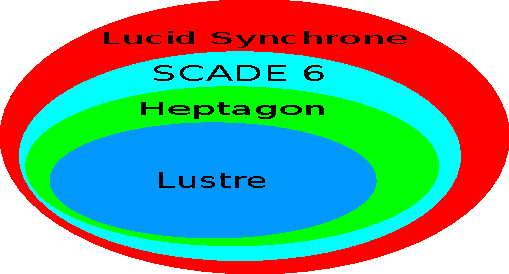
\includegraphics[scale=0.65]{comparo.pdf}
  \end{center}

  Les traits marquants d'\heptagon{} sont :

  \begin{itemize}
  \item Les programmes sont structurés en noeuds contenants des équations de
    suites ou des automates.
  \item Le processus de compilation vérifie des propriétés de sûreté et raffine
    le programme jusqu'à générer du code impératif (e.g. langage C).
  \item<alert@2-> Il est possible de générer du code VHDL.
  \end{itemize}
\end{frame}

\begin{frame}
  \frametitle{Génération de code VHDL}

  \begin{center}
    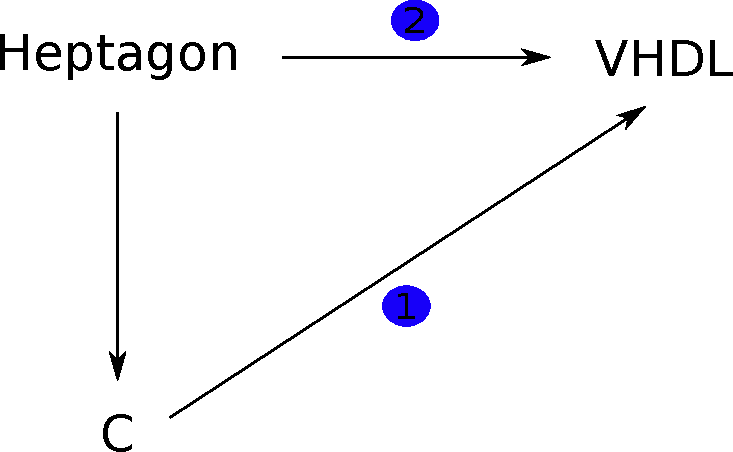
\includegraphics[scale=0.4]{sens_traduction.pdf}
  \end{center}

  Pour produire du code VHDL, deux points de départ sont possibles :

  \begin{enumerate}
  \item Le code C produit par le compilateur original (\scade{} ou
    \heptagon{}). Cette approche est celle de la société GeenSoft.
  \item La représentation intermédiaire à flots de données interne au
    compilateur du langage synchrone.
  \end{enumerate}

  \pause

  Nous avons retenu le second cheminement, et l'avons clairement spécifié afin
  de pouvoir envisager une certification DO-178B ultérieure.
\end{frame}

\begin{frame}
  \frametitle{Exemple 1 : compteur - code original}

  \begin{Verbatim}[commandchars=\\\{\}]
\PY{k+kd}{node}\PY{+w}{ }\PY{n}{compteur}\PY{p}{(}\PY{n}{tick}\PY{p}{,}\PY{+w}{ }\PY{n}{top}\PY{+w}{ }\PY{p}{:}\PY{+w}{ }\PY{k+kt}{bool}\PY{p}{)}\PY{+w}{ }\PY{k}{returns}\PY{+w}{ }\PY{p}{(}\PY{n}{o}\PY{+w}{ }\PY{p}{:}\PY{+w}{ }\PY{k+kt}{int}\PY{p}{)}
\PY{k+kd}{var}\PY{+w}{ }\PY{o}{pre}\PY{n}{s}\PY{+w}{ }\PY{p}{:}\PY{+w}{ }\PY{k+kt}{int}\PY{p}{;}
\PY{k}{let}
\PY{+w}{ }\PY{+w}{ }\PY{o}{pre}\PY{n}{s}\PY{+w}{ }\PY{o}{=}\PY{+w}{ }\PY{k}{if}\PY{+w}{ }\PY{n}{tick}\PY{+w}{ }\PY{k}{then}\PY{+w}{ }\PY{l+m+mi}{1}\PY{+w}{ }\PY{k}{else}\PY{+w}{ }\PY{l+m+mi}{0}\PY{p}{;}
\PY{+w}{ }\PY{+w}{ }\PY{n}{reset}\PY{+w}{ }\PY{n}{o}\PY{+w}{ }\PY{o}{=}\PY{+w}{ }\PY{p}{(}\PY{l+m+mi}{0}\PY{+w}{ }\PY{k}{fby}\PY{+w}{ }\PY{n}{o}\PY{p}{)}\PY{+w}{ }\PY{o}{+}\PY{+w}{ }\PY{o}{pre}\PY{n}{s}\PY{+w}{ }\PY{n}{every}\PY{+w}{ }\PY{n}{top}\PY{p}{;}
\PY{k}{tel}

\PY{k+kd}{node}\PY{+w}{ }\PY{n}{main}\PY{p}{(}\PY{p}{)}\PY{+w}{ }\PY{k}{returns}\PY{+w}{ }\PY{p}{(}\PY{n}{o}\PY{+w}{ }\PY{p}{:}\PY{+w}{ }\PY{k+kt}{int}\PY{p}{)}
\PY{k}{let}
\PY{+w}{ }\PY{+w}{ }\PY{n}{o}\PY{+w}{ }\PY{o}{=}\PY{+w}{ }\PY{n}{compteur}\PY{p}{(}\PY{l}{true}\PY{+w}{ }\PY{+w}{ }\PY{k}{fby}\PY{+w}{ }\PY{+w}{ }\PY{l}{true}\PY{+w}{ }\PY{k}{fby}\PY{+w}{ }\PY{l}{false}\PY{+w}{ }\PY{k}{fby}\PY{+w}{ }\PY{l}{true}\PY{p}{,}
\PY{+w}{ }\PY{+w}{ }\PY{+w}{ }\PY{+w}{ }\PY{+w}{ }\PY{+w}{ }\PY{+w}{ }\PY{+w}{ }\PY{+w}{ }\PY{+w}{ }\PY{+w}{ }\PY{+w}{ }\PY{+w}{ }\PY{+w}{ }\PY{+w}{ }\PY{l}{false}\PY{+w}{ }\PY{k}{fby}\PY{+w}{ }\PY{l}{false}\PY{+w}{ }\PY{k}{fby}\PY{+w}{ }\PY{l}{true}\PY{+w}{ }\PY{k}{fby}\PY{+w}{ }\PY{l}{false}\PY{p}{)}\PY{p}{;}
\PY{k}{tel}
\end{Verbatim}

\end{frame}


\begin{frame}
  \frametitle{Exemple 1 : compteur - exemple de sortie attendue}

  \[
  \begin{array}{r|llllllllllllllllllllllllllll}
    \hline
    tick & t & t & t & f & \dots \\
    \hline
    top & f & f & t & f & \dots \\
    \hline
    o & 1 & 2 & 1 & 1 & \dots \\
    \hline
  \end{array}
  \]
\end{frame}


\begin{frame}
  \frametitle{Exemple 1 : compteur - code MiniLS}

  \footnotesize

  \begin{Verbatim}[commandchars=\\\{\}]
\PY{k+kd}{node}\PY{+w}{ }\PY{n}{compteur}\PY{p}{(}\PY{n}{tick}\PY{+w}{ }\PY{p}{:}\PY{+w}{ }\PY{k+kt}{bool}\PY{p}{;}\PY{+w}{ }\PY{n}{top}\PY{+w}{ }\PY{p}{:}\PY{+w}{ }\PY{k+kt}{bool}\PY{p}{)}\PY{+w}{ }\PY{k}{returns}\PY{+w}{ }\PY{p}{(}\PY{n}{o}\PY{+w}{ }\PY{p}{:}\PY{+w}{ }\PY{k+kt}{int}\PY{p}{)}
\PY{k+kd}{var}\PY{+w}{ }\PY{o}{pre}\PY{n}{s}\PY{+w}{ }\PY{p}{:}\PY{+w}{ }\PY{k+kt}{int}\PY{p}{;}
\PY{k}{let}
\PY{+w}{ }\PY{+w}{ }\PY{n}{o}\PY{+w}{ }\PY{o}{=}\PY{+w}{ }\PY{p}{(}\PY{k}{if}\PY{+w}{ }\PY{n}{top}\PY{+w}{ }\PY{k}{then}\PY{+w}{ }\PY{l+m+mi}{0}\PY{+w}{ }\PY{k}{else}\PY{+w}{ }\PY{l+m+mi}{0}\PY{+w}{ }\PY{k}{fby}\PY{+w}{ }\PY{n}{o}\PY{p}{)}\PY{+w}{ }\PY{o}{+}\PY{+w}{ }\PY{o}{pre}\PY{n}{s}\PY{p}{;}
\PY{+w}{ }\PY{+w}{ }\PY{o}{pre}\PY{n}{s}\PY{+w}{ }\PY{o}{=}\PY{+w}{ }\PY{k}{if}\PY{+w}{ }\PY{n}{tick}\PY{+w}{ }\PY{k}{then}\PY{+w}{ }\PY{l+m+mi}{1}\PY{+w}{ }\PY{k}{else}\PY{+w}{ }\PY{l+m+mi}{0}
\PY{k}{tel}
\end{Verbatim}


  Le code n'est plus formé que d'équations.
\end{frame}

\begin{frame}
  \frametitle{Exemple 1 : compteur - code MiniLS sans reset}

  \footnotesize

  \begin{Verbatim}[commandchars=\\\{\}]
\PY{k+kd}{node}\PY{+w}{ }\PY{n}{compteur}\PY{p}{(}\PY{n}{rst\PYZus{}2}\PY{+w}{ }\PY{p}{:}\PY{+w}{ }\PY{k+kt}{bool}\PY{p}{;}\PY{+w}{ }\PY{n}{tick}\PY{+w}{ }\PY{p}{:}\PY{+w}{ }\PY{k+kt}{bool}\PY{p}{;}\PY{+w}{ }\PY{n}{top}\PY{+w}{ }\PY{p}{:}\PY{+w}{ }\PY{k+kt}{bool}\PY{p}{)}
\PY{+w}{ }\PY{+w}{ }\PY{+w}{ }\PY{+w}{ }\PY{+w}{ }\PY{k}{returns}\PY{+w}{ }\PY{p}{(}\PY{n}{o}\PY{+w}{ }\PY{p}{:}\PY{+w}{ }\PY{k+kt}{int}\PY{p}{)}
\PY{k}{let}
\PY{+w}{ }\PY{+w}{ }\PY{n}{o}\PY{+w}{ }\PY{o}{=}\PY{+w}{ }\PY{p}{(}\PY{k}{if}\PY{+w}{ }\PY{n}{top}\PY{+w}{ }\PY{k}{then}\PY{+w}{ }\PY{l+m+mi}{0}\PY{+w}{ }\PY{k}{else}\PY{+w}{ }\PY{p}{(}\PY{k}{if}\PY{+w}{ }\PY{n}{rst\PYZus{}2}\PY{+w}{ }\PY{k}{then}\PY{+w}{ }\PY{l+m+mi}{0}\PY{+w}{ }\PY{k}{else}\PY{+w}{ }\PY{p}{(}\PY{l+m+mi}{0}\PY{+w}{ }\PY{k}{fby}\PY{+w}{ }\PY{n}{o}\PY{p}{)}\PY{p}{)}\PY{p}{)}
\PY{+w}{ }\PY{+w}{ }\PY{+w}{ }\PY{+w}{ }\PY{o}{+}\PY{+w}{ }\PY{p}{(}\PY{k}{if}\PY{+w}{ }\PY{n}{tick}\PY{+w}{ }\PY{k}{then}\PY{+w}{ }\PY{l+m+mi}{1}\PY{+w}{ }\PY{k}{else}\PY{+w}{ }\PY{l+m+mi}{0}\PY{p}{)}
\PY{k}{tel}
\end{Verbatim}


  La réinitialisation logique est explicitée via un paramètre du nœud.
\end{frame}

\begin{frame}
  \frametitle{Exemple 1 : compteur - code MiniLS final}

  \footnotesize

  \begin{Verbatim}[commandchars=\\\{\}]
\PY{k+kd}{node}\PY{+w}{ }\PY{n}{compteur}\PY{p}{(}\PY{n}{rst\PYZus{}2}\PY{+w}{ }\PY{p}{:}\PY{+w}{ }\PY{k+kt}{bool}\PY{p}{;}\PY{+w}{ }\PY{n}{tick}\PY{+w}{ }\PY{p}{:}\PY{+w}{ }\PY{k+kt}{bool}\PY{p}{;}\PY{+w}{ }\PY{n}{top}\PY{+w}{ }\PY{p}{:}\PY{+w}{ }\PY{k+kt}{bool}\PY{p}{)}\PY{+w}{ }\PY{k}{returns}\PY{+w}{ }\PY{p}{(}\PY{n}{o}\PY{+w}{ }\PY{p}{:}\PY{+w}{ }\PY{k+kt}{int}\PY{p}{)}
\PY{k+kd}{var}\PY{+w}{ }\PY{n}{\PYZus{}v\PYZus{}28}\PY{+w}{ }\PY{p}{:}\PY{+w}{ }\PY{k+kt}{int}\PY{p}{;}\PY{+w}{ }\PY{n}{\PYZus{}v\PYZus{}27}\PY{+w}{ }\PY{p}{:}\PY{+w}{ }\PY{k+kt}{int}\PY{p}{;}\PY{+w}{ }\PY{n}{\PYZus{}v\PYZus{}26}\PY{+w}{ }\PY{p}{:}\PY{+w}{ }\PY{k+kt}{int}\PY{p}{;}
\PY{k}{let}
\PY{+w}{ }\PY{+w}{ }\PY{n}{\PYZus{}v\PYZus{}27}\PY{+w}{ }\PY{o}{=}
\PY{+w}{ }\PY{+w}{ }\PY{+w}{ }\PY{+w}{ }\PY{k}{merge}\PY{+w}{ }\PY{n}{top}
\PY{+w}{ }\PY{+w}{ }\PY{+w}{ }\PY{+w}{ }\PY{+w}{ }\PY{+w}{ }\PY{p}{(}\PY{l}{true}\PY{+w}{ }\PY{o}{->}\PY{+w}{ }\PY{p}{(}\PY{l+m+mi}{0}\PY{+w}{ }\PY{k}{when}\PY{+w}{ }\PY{l}{true}\PY{p}{(}\PY{n}{top}\PY{p}{)}\PY{p}{)}\PY{p}{)}
\PY{+w}{ }\PY{+w}{ }\PY{+w}{ }\PY{+w}{ }\PY{+w}{ }\PY{+w}{ }\PY{p}{(}\PY{l}{false}\PY{+w}{ }\PY{o}{->}
\PY{+w}{ }\PY{+w}{ }\PY{+w}{ }\PY{+w}{ }\PY{+w}{ }\PY{+w}{ }\PY{+w}{ }\PY{+w}{ }\PY{p}{(}\PY{k}{merge}\PY{+w}{ }\PY{n}{rst\PYZus{}2}
\PY{+w}{ }\PY{+w}{ }\PY{+w}{ }\PY{+w}{ }\PY{+w}{ }\PY{+w}{ }\PY{+w}{ }\PY{+w}{ }\PY{+w}{ }\PY{+w}{ }\PY{+w}{ }\PY{p}{(}\PY{l}{true}\PY{+w}{ }\PY{o}{->}\PY{+w}{ }\PY{p}{(}\PY{l+m+mi}{0}\PY{+w}{ }\PY{k}{when}\PY{+w}{ }\PY{l}{true}\PY{p}{(}\PY{n}{rst\PYZus{}2}\PY{p}{)}\PY{p}{)}\PY{p}{)}
\PY{+w}{ }\PY{+w}{ }\PY{+w}{ }\PY{+w}{ }\PY{+w}{ }\PY{+w}{ }\PY{+w}{ }\PY{+w}{ }\PY{+w}{ }\PY{+w}{ }\PY{+w}{ }\PY{p}{(}\PY{l}{false}\PY{+w}{ }\PY{o}{->}\PY{+w}{ }\PY{p}{(}\PY{n}{\PYZus{}v\PYZus{}26}\PY{+w}{ }\PY{k}{when}\PY{+w}{ }\PY{l}{false}\PY{p}{(}\PY{n}{rst\PYZus{}2}\PY{p}{)}\PY{p}{)}\PY{p}{)}
\PY{+w}{ }\PY{+w}{ }\PY{+w}{ }\PY{+w}{ }\PY{+w}{ }\PY{+w}{ }\PY{+w}{ }\PY{+w}{ }\PY{+w}{ }\PY{k}{when}\PY{+w}{ }\PY{l}{false}\PY{p}{(}\PY{n}{top}\PY{p}{)}\PY{p}{)}\PY{p}{)}\PY{p}{;}
\PY{+w}{ }\PY{+w}{ }\PY{n}{\PYZus{}v\PYZus{}28}\PY{+w}{ }\PY{o}{=}\PY{+w}{ }\PY{k}{merge}\PY{+w}{ }\PY{n}{tick}\PY{+w}{ }\PY{p}{(}\PY{l}{true}\PY{+w}{ }\PY{o}{->}\PY{+w}{ }\PY{p}{(}\PY{l+m+mi}{1}\PY{+w}{ }\PY{k}{when}\PY{+w}{ }\PY{l}{true}\PY{p}{(}\PY{n}{tick}\PY{p}{)}\PY{p}{)}\PY{p}{)}
\PY{+w}{ }\PY{+w}{ }\PY{+w}{ }\PY{+w}{ }\PY{+w}{ }\PY{+w}{ }\PY{+w}{ }\PY{+w}{ }\PY{+w}{ }\PY{+w}{ }\PY{+w}{ }\PY{+w}{ }\PY{+w}{ }\PY{+w}{ }\PY{+w}{ }\PY{+w}{ }\PY{+w}{ }\PY{+w}{ }\PY{+w}{ }\PY{+w}{ }\PY{+w}{ }\PY{p}{(}\PY{l}{false}\PY{+w}{ }\PY{o}{->}\PY{+w}{ }\PY{p}{(}\PY{l+m+mi}{0}\PY{+w}{ }\PY{k}{when}\PY{+w}{ }\PY{l}{false}\PY{p}{(}\PY{n}{tick}\PY{p}{)}\PY{p}{)}\PY{p}{)}\PY{p}{;}
\PY{+w}{ }\PY{+w}{ }\PY{n}{o}\PY{+w}{ }\PY{o}{=}\PY{+w}{ }\PY{n}{\PYZus{}v\PYZus{}27}\PY{+w}{ }\PY{o}{+}\PY{+w}{ }\PY{n}{\PYZus{}v\PYZus{}28}\PY{p}{;}
\PY{+w}{ }\PY{+w}{ }\PY{n}{\PYZus{}v\PYZus{}26}\PY{+w}{ }\PY{o}{=}\PY{+w}{ }\PY{l+m+mi}{0}\PY{+w}{ }\PY{k}{fby}\PY{+w}{ }\PY{n}{o}
\PY{k}{tel}
\end{Verbatim}


  Le code est normalisé et ordonnancé.
\end{frame}

\begin{frame}
  \frametitle{Exemple 1 : compteur - code VHDL}

  \tiny

  \begin{columns}[t]
    \hspace{1cm}
    \begin{column}{6cm}
      \begin{Verbatim}[commandchars=\\\{\}]
\PY{k+kn}{use}\PY{+w}{ }\PY{n}{work}\PY{o}{.}\PY{n}{compteur}\PY{o}{.}\PY{n}{all}\PY{p}{;}

\PY{k+kn}{library}\PY{+w}{ }\PY{n}{ieee}\PY{p}{;}
\PY{k+kn}{use}\PY{+w}{ }\PY{n}{ieee}\PY{o}{.}\PY{k+kt}{std\PYZus{}logic}\PY{n}{\PYZus{}1164}\PY{o}{.}\PY{n}{all}\PY{p}{;}

\PY{k+kd}{entity}\PY{+w}{ }\PY{n}{compteur}\PY{+w}{ }\PY{k}{is}
\PY{+w}{ }\PY{+w}{ }\PY{k}{port}\PY{+w}{ }\PY{p}{(}\PY{k+kd}{signal}\PY{+w}{ }\PY{n}{clk\PYZus{}1}\PY{+w}{ }\PY{p}{:}\PY{+w}{ }\PY{n}{in}\PY{+w}{ }\PY{k+kt}{std\PYZus{}logic}\PY{p}{;}\PY{+w}{ }
\PY{+w}{ }\PY{+w}{ }\PY{+w}{ }\PY{+w}{ }\PY{+w}{ }\PY{+w}{ }\PY{+w}{ }\PY{+w}{ }\PY{k+kd}{signal}\PY{+w}{ }\PY{n}{hw\PYZus{}rst\PYZus{}3}\PY{+w}{ }\PY{p}{:}\PY{+w}{ }\PY{n}{in}\PY{+w}{ }\PY{k+kt}{std\PYZus{}logic}\PY{p}{;}
\PY{+w}{ }\PY{+w}{ }\PY{+w}{ }\PY{+w}{ }\PY{+w}{ }\PY{+w}{ }\PY{+w}{ }\PY{+w}{ }\PY{k+kd}{signal}\PY{+w}{ }\PY{n}{rst\PYZus{}2}\PY{+w}{ }\PY{p}{:}\PY{+w}{ }\PY{n}{in}\PY{+w}{ }\PY{k+kt}{std\PYZus{}logic}\PY{p}{;}\PY{+w}{ }
\PY{+w}{ }\PY{+w}{ }\PY{+w}{ }\PY{+w}{ }\PY{+w}{ }\PY{+w}{ }\PY{+w}{ }\PY{+w}{ }\PY{k+kd}{signal}\PY{+w}{ }\PY{n}{tick}\PY{+w}{ }\PY{p}{:}\PY{+w}{ }\PY{n}{in}\PY{+w}{ }\PY{k+kt}{std\PYZus{}logic}\PY{p}{;}
\PY{+w}{ }\PY{+w}{ }\PY{+w}{ }\PY{+w}{ }\PY{+w}{ }\PY{+w}{ }\PY{+w}{ }\PY{+w}{ }\PY{k+kd}{signal}\PY{+w}{ }\PY{n}{top}\PY{+w}{ }\PY{p}{:}\PY{+w}{ }\PY{n}{in}\PY{+w}{ }\PY{k+kt}{std\PYZus{}logic}\PY{p}{;}
\PY{+w}{ }\PY{+w}{ }\PY{+w}{ }\PY{+w}{ }\PY{+w}{ }\PY{+w}{ }\PY{+w}{ }\PY{+w}{ }\PY{k+kd}{signal}\PY{+w}{ }\PY{n}{o\PYZus{}o}\PY{+w}{ }\PY{p}{:}\PY{+w}{ }\PY{n}{out}\PY{+w}{ }\PY{k+kt}{integer}\PY{p}{)}\PY{p}{;}
\PY{k}{end}\PY{+w}{ }\PY{k+kd}{entity}\PY{+w}{ }\PY{n}{compteur}\PY{p}{;}

\PY{k+kd}{architecture}\PY{+w}{ }\PY{n}{rtl}\PY{+w}{ }\PY{k}{of}\PY{+w}{ }\PY{n}{compteur}\PY{+w}{ }\PY{k}{is}
\PY{+w}{ }\PY{+w}{ }\PY{k+kd}{signal}\PY{+w}{ }\PY{n}{h\PYZus{}v\PYZus{}26}\PY{+w}{ }\PY{p}{:}\PY{+w}{ }\PY{k+kt}{integer}\PY{p}{;}
\PY{k}{begin}
\PY{+w}{ }\PY{+w}{ }\PY{n}{update}\PY{+w}{ }\PY{p}{:}\PY{+w}{ }\PY{k+kd}{process}\PY{+w}{ }\PY{p}{(}\PY{n}{clk\PYZus{}1}\PY{p}{,}\PY{+w}{ }\PY{n}{hw\PYZus{}rst\PYZus{}3}\PY{p}{,}\PY{+w}{ }\PY{n}{rst\PYZus{}2}\PY{p}{,}
\PY{+w}{ }\PY{+w}{ }\PY{+w}{ }\PY{+w}{ }\PY{+w}{ }\PY{+w}{ }\PY{+w}{ }\PY{+w}{ }\PY{+w}{ }\PY{+w}{ }\PY{+w}{ }\PY{+w}{ }\PY{+w}{ }\PY{+w}{ }\PY{+w}{ }\PY{+w}{ }\PY{+w}{ }\PY{+w}{ }\PY{+w}{ }\PY{+w}{ }\PY{n}{tick}\PY{p}{,}\PY{+w}{ }\PY{n}{top}\PY{p}{,}\PY{+w}{ }\PY{n}{h\PYZus{}v\PYZus{}26}\PY{p}{)}
\PY{+w}{ }\PY{+w}{ }\PY{+w}{ }\PY{+w}{ }\PY{k+kd}{variable}\PY{+w}{ }\PY{n}{h\PYZus{}v\PYZus{}27}\PY{+w}{ }\PY{p}{:}\PY{+w}{ }\PY{k+kt}{integer}\PY{p}{;}
\PY{+w}{ }\PY{+w}{ }\PY{+w}{ }\PY{+w}{ }\PY{k+kd}{variable}\PY{+w}{ }\PY{n}{h\PYZus{}v\PYZus{}28}\PY{+w}{ }\PY{p}{:}\PY{+w}{ }\PY{k+kt}{integer}\PY{p}{;}
\PY{+w}{ }\PY{+w}{ }\PY{+w}{ }\PY{+w}{ }\PY{k+kd}{variable}\PY{+w}{ }\PY{n}{o}\PY{+w}{ }\PY{p}{:}\PY{+w}{ }\PY{k+kt}{integer}\PY{p}{;}
\PY{+w}{ }\PY{+w}{ }\PY{k}{begin}
\PY{+w}{ }\PY{+w}{ }\PY{+w}{ }\PY{+w}{ }\PY{k}{case}\PY{+w}{ }\PY{n}{top}\PY{+w}{ }\PY{k}{is}
\PY{+w}{ }\PY{+w}{ }\PY{+w}{ }\PY{+w}{ }\PY{+w}{ }\PY{+w}{ }\PY{k}{when}\PY{+w}{ }\PY{p}{'}\PY{l+m+mi}{1}\PY{p}{'}\PY{+w}{ }\PY{p}{=>}\PY{+w}{ }\PY{n}{h\PYZus{}v\PYZus{}27}\PY{+w}{ }\PY{p}{:}\PY{o}{=}\PY{+w}{ }\PY{l+m+mi}{0}\PY{p}{;}
\PY{+w}{ }\PY{+w}{ }\PY{+w}{ }\PY{+w}{ }\PY{+w}{ }\PY{+w}{ }\PY{k}{when}\PY{+w}{ }\PY{p}{'}\PY{l+m+mi}{0}\PY{p}{'}\PY{+w}{ }\PY{p}{=>}\PY{+w}{ }\PY{k}{case}\PY{+w}{ }\PY{n}{rst\PYZus{}2}\PY{+w}{ }\PY{k}{is}
\PY{+w}{ }\PY{+w}{ }\PY{+w}{ }\PY{+w}{ }\PY{+w}{ }\PY{+w}{ }\PY{+w}{ }\PY{+w}{ }\PY{+w}{ }\PY{+w}{ }\PY{+w}{ }\PY{+w}{ }\PY{+w}{ }\PY{+w}{ }\PY{+w}{ }\PY{+w}{ }\PY{+w}{ }\PY{+w}{ }\PY{+w}{ }\PY{+w}{ }\PY{k}{when}\PY{+w}{ }\PY{p}{'}\PY{l+m+mi}{1}\PY{p}{'}\PY{+w}{ }\PY{p}{=>}\PY{+w}{ }\PY{n}{h\PYZus{}v\PYZus{}27}\PY{+w}{ }\PY{p}{:}\PY{o}{=}\PY{+w}{ }\PY{l+m+mi}{0}\PY{p}{;}
\PY{+w}{ }\PY{+w}{ }\PY{+w}{ }\PY{+w}{ }\PY{+w}{ }\PY{+w}{ }\PY{+w}{ }\PY{+w}{ }\PY{+w}{ }\PY{+w}{ }\PY{+w}{ }\PY{+w}{ }\PY{+w}{ }\PY{+w}{ }\PY{+w}{ }\PY{+w}{ }\PY{+w}{ }\PY{+w}{ }\PY{+w}{ }\PY{+w}{ }\PY{k}{when}\PY{+w}{ }\PY{p}{'}\PY{l+m+mi}{0}\PY{p}{'}\PY{+w}{ }\PY{p}{=>}\PY{+w}{ }\PY{n}{h\PYZus{}v\PYZus{}27}\PY{+w}{ }\PY{p}{:}\PY{o}{=}\PY{+w}{ }\PY{n}{h\PYZus{}v\PYZus{}26}\PY{p}{;}
\PY{+w}{ }\PY{+w}{ }\PY{+w}{ }\PY{+w}{ }\PY{+w}{ }\PY{+w}{ }\PY{+w}{ }\PY{+w}{ }\PY{+w}{ }\PY{+w}{ }\PY{+w}{ }\PY{+w}{ }\PY{+w}{ }\PY{+w}{ }\PY{+w}{ }\PY{+w}{ }\PY{+w}{ }\PY{+w}{ }\PY{k}{end}\PY{+w}{ }\PY{k}{case}\PY{p}{;}
\PY{+w}{ }\PY{+w}{ }\PY{+w}{ }\PY{+w}{ }\PY{k}{end}\PY{+w}{ }\PY{k}{case}\PY{p}{;}
\end{Verbatim}

    \end{column}
    \begin{column}{6cm}
      \begin{Verbatim}[commandchars=\\\{\}]
\PY{+w}{ }\PY{+w}{ }\PY{+w}{ }\PY{+w}{ }\PY{n}{case}\PY{+w}{ }\PY{n}{tick}\PY{+w}{ }\PY{n}{is}
\PY{+w}{ }\PY{+w}{ }\PY{+w}{ }\PY{+w}{ }\PY{+w}{ }\PY{+w}{ }\PY{k}{when}\PY{+w}{ }\PY{p}{'}\PY{l+m+mi}{1}\PY{p}{'}\PY{+w}{ }\PY{p}{=>}\PY{+w}{ }\PY{n}{h\PYZus{}v\PYZus{}28}\PY{+w}{ }\PY{p}{:}\PY{o}{=}\PY{+w}{ }\PY{l+m+mi}{1}\PY{p}{;}
\PY{+w}{ }\PY{+w}{ }\PY{+w}{ }\PY{+w}{ }\PY{+w}{ }\PY{+w}{ }\PY{k}{when}\PY{+w}{ }\PY{p}{'}\PY{l+m+mi}{0}\PY{p}{'}\PY{+w}{ }\PY{p}{=>}\PY{+w}{ }\PY{n}{h\PYZus{}v\PYZus{}28}\PY{+w}{ }\PY{p}{:}\PY{o}{=}\PY{+w}{ }\PY{l+m+mi}{0}\PY{p}{;}
\PY{+w}{ }\PY{+w}{ }\PY{+w}{ }\PY{+w}{ }\PY{k}{end}\PY{+w}{ }\PY{n}{case}\PY{p}{;}
\PY{+w}{ }\PY{+w}{ }\PY{+w}{ }\PY{+w}{ }\PY{n}{o}\PY{+w}{ }\PY{p}{:}\PY{o}{=}\PY{+w}{ }\PY{p}{(}\PY{n}{h\PYZus{}v\PYZus{}27}\PY{+w}{ }\PY{o}{+}\PY{+w}{ }\PY{n}{h\PYZus{}v\PYZus{}28}\PY{p}{)}\PY{p}{;}
\PY{+w}{ }\PY{+w}{ }\PY{+w}{ }\PY{+w}{ }\PY{k}{if}\PY{+w}{ }\PY{p}{(}\PY{n}{hw\PYZus{}rst\PYZus{}3}\PY{+w}{ }\PY{o}{=}\PY{+w}{ }\PY{p}{'}\PY{l+m+mi}{1}\PY{p}{'}\PY{p}{)}\PY{+w}{ }\PY{k}{then}
\PY{+w}{ }\PY{+w}{ }\PY{+w}{ }\PY{+w}{ }\PY{+w}{ }\PY{+w}{ }\PY{n}{h\PYZus{}v\PYZus{}26}\PY{+w}{ }\PY{o}{<=}\PY{+w}{ }\PY{l+m+mi}{0}\PY{p}{;}
\PY{+w}{ }\PY{+w}{ }\PY{+w}{ }\PY{+w}{ }\PY{k}{elsif}\PY{+w}{ }\PY{n}{rising\PYZus{}edge}\PY{p}{(}\PY{n}{clk\PYZus{}1}\PY{p}{)}\PY{+w}{ }\PY{k}{then}
\PY{+w}{ }\PY{+w}{ }\PY{+w}{ }\PY{+w}{ }\PY{+w}{ }\PY{+w}{ }\PY{n}{h\PYZus{}v\PYZus{}26}\PY{+w}{ }\PY{o}{<=}\PY{+w}{ }\PY{n}{o}\PY{p}{;}
\PY{+w}{ }\PY{+w}{ }\PY{+w}{ }\PY{+w}{ }\PY{k}{end}\PY{+w}{ }\PY{k}{if}\PY{p}{;}
\PY{+w}{ }\PY{+w}{ }\PY{+w}{ }\PY{+w}{ }\PY{n}{o\PYZus{}o}\PY{+w}{ }\PY{o}{<=}\PY{+w}{ }\PY{n}{o}\PY{p}{;}
\PY{+w}{ }\PY{+w}{ }\PY{k}{end}\PY{+w}{ }\PY{k+kd}{process}\PY{+w}{ }\PY{n}{update}\PY{p}{;}
\PY{k}{end}\PY{+w}{ }\PY{k+kd}{architecture}\PY{+w}{ }\PY{n}{rtl}\PY{p}{;}
\end{Verbatim}

    \end{column}
  \end{columns}
\end{frame}

\begin{frame}
  \frametitle{Exemple 1 : compteur - caractéristiques du code VHDL}

  \begin{block}{Simulation comportementale}
    \vspace{0.3cm}
    \begin{center}
      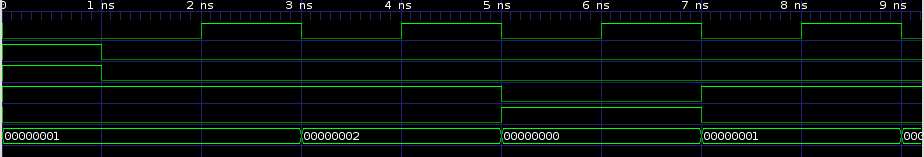
\includegraphics[width=10cm]{capture-chrono-compteur}
    \end{center}
  \end{block}

  \begin{block}{Synthèse}
    L'outil industriel \textit{Xilinx XST} synthétise une netlist avec des
    propriétés satisfaisantes :

    \begin{itemize}
    \item Un additionneur 32 bits pour \textbf{o}.
    \item Un registre 32 bits pour \textbf{h\_v\_26}.
    \end{itemize}
  \end{block}
\end{frame}


\begin{frame}
  \frametitle{Exemple 2 : compteur de bits - code original}

  \footnotesize

  \begin{Verbatim}[commandchars=\\\{\}]
\PY{k+kd}{node}\PY{+w}{ }\PY{n}{countbits}\PY{p}{(}\PY{n}{x}\PY{+w}{ }\PY{p}{:}\PY{+w}{ }\PY{k+kt}{bool}\PY{o}{\PYZca{}}\PY{n}{n}\PY{p}{;}\PY{+w}{ }\PY{n}{mask}\PY{+w}{ }\PY{p}{:}\PY{+w}{ }\PY{k+kt}{bool}\PY{o}{\PYZca{}}\PY{n}{n}\PY{p}{;}\PY{+w}{ }\PY{n}{sw\PYZus{}mode}\PY{+w}{ }\PY{p}{:}\PY{+w}{ }\PY{k+kt}{bool}\PY{p}{)}
\PY{+w}{ }\PY{+w}{ }\PY{+w}{ }\PY{+w}{ }\PY{+w}{ }\PY{+w}{ }\PY{k}{returns}\PY{+w}{ }\PY{p}{(}\PY{n}{o}\PY{+w}{ }\PY{p}{:}\PY{+w}{ }\PY{k+kt}{int}\PY{p}{)}
\PY{k+kd}{var}\PY{+w}{ }\PY{n}{bits}\PY{+w}{ }\PY{p}{:}\PY{+w}{ }\PY{k+kt}{bool}\PY{o}{\PYZca{}}\PY{n}{n}\PY{p}{;}
\PY{k}{let}
\PY{+w}{ }\PY{+w}{ }\PY{k}{automaton}
\PY{+w}{ }\PY{+w}{ }\PY{+w}{ }\PY{+w}{ }\PY{k}{state}\PY{+w}{ }\PY{l+s+ss}{Simple}
\PY{+w}{ }\PY{+w}{ }\PY{+w}{ }\PY{+w}{ }\PY{+w}{ }\PY{+w}{ }\PY{k}{do}\PY{+w}{ }\PY{n}{bits}\PY{+w}{ }\PY{o}{=}\PY{+w}{ }\PY{n}{x}\PY{p}{;}
\PY{+w}{ }\PY{+w}{ }\PY{+w}{ }\PY{+w}{ }\PY{+w}{ }\PY{+w}{ }\PY{k}{unless}\PY{+w}{ }\PY{n}{sw\PYZus{}mode}\PY{+w}{ }\PY{k}{then}\PY{+w}{ }\PY{l+s+ss}{Masked}
\PY{+w}{ }\PY{+w}{ }\PY{+w}{ }\PY{+w}{ }\PY{k}{state}\PY{+w}{ }\PY{l+s+ss}{Masked}
\PY{+w}{ }\PY{+w}{ }\PY{+w}{ }\PY{+w}{ }\PY{+w}{ }\PY{+w}{ }\PY{k}{do}\PY{+w}{ }\PY{n}{bits}\PY{+w}{ }\PY{o}{=}\PY{+w}{ }\PY{k}{map}\PY{+w}{ }\PY{p}{(}\PY{o}{&}\PY{p}{)}\PY{+w}{ }\PY{p}{<}\PY{p}{<}\PY{n}{n}\PY{p}{>}\PY{p}{>}\PY{p}{(}\PY{n}{x}\PY{p}{,}\PY{+w}{ }\PY{n}{mask}\PY{p}{)}\PY{p}{;}
\PY{+w}{ }\PY{+w}{ }\PY{+w}{ }\PY{+w}{ }\PY{+w}{ }\PY{+w}{ }\PY{k}{unless}\PY{+w}{ }\PY{n}{sw\PYZus{}mode}\PY{+w}{ }\PY{k}{then}\PY{+w}{ }\PY{l+s+ss}{Simple}
\PY{+w}{ }\PY{+w}{ }\PY{k}{end}\PY{p}{;}

\PY{+w}{ }\PY{+w}{ }\PY{n}{o}\PY{+w}{ }\PY{o}{=}\PY{+w}{ }\PY{k}{fold}\PY{+w}{ }\PY{p}{(}\PY{o}{+}\PY{p}{)}\PY{+w}{ }\PY{p}{<}\PY{p}{<}\PY{n}{n}\PY{p}{>}\PY{p}{>}\PY{+w}{ }\PY{p}{(}\PY{k}{map}\PY{+w}{ }\PY{k+kt}{int}\PY{n}{\PYZus{}of\PYZus{}bool}\PY{+w}{ }\PY{p}{<}\PY{p}{<}\PY{n}{n}\PY{p}{>}\PY{p}{>}\PY{p}{(}\PY{n}{bits}\PY{p}{)}\PY{p}{,}\PY{+w}{ }\PY{l+m+mi}{0}\PY{p}{)}\PY{p}{;}
\PY{k}{tel}
\end{Verbatim}

\end{frame}

\begin{frame}
  \frametitle{Exemple 2 : compteur de bits - exemple de sortie attendue}

  Ici, $n = 3$.

  \[
  \begin{array}{r|llllllllllllllllllllllllllll}
    \hline
    x & [t,f,f] & [t,t,t] & [t,t,t] & [t,t,t] & \dots \\
    \hline
    mask & [t,f,t] & [t,f,t] & [t,f,t] & [t,f,t] & \dots \\
    \hline
    sw\_mode & f & t & t & f & \dots \\
    \hline
    o & 1 & 2 & 3 & 3 & \dots \\
    \hline
  \end{array}
  \]
\end{frame}

\begin{frame}
  \frametitle{Exemple 2 : compteur de bits - code MiniLS}

  \tiny

  \begin{columns}[t]
    \hspace{1cm}
    \begin{column}{6cm}
      \begin{Verbatim}[commandchars=\\\{\}]
\PY{k+kd}{node}\PY{+w}{ }\PY{n}{countbits}\PY{p}{(}\PY{n}{x}\PY{+w}{ }\PY{p}{:}\PY{+w}{ }\PY{k+kt}{bool}\PY{o}{\PYZca{}}\PY{n}{n}\PY{p}{;}\PY{+w}{ }\PY{n}{mask}\PY{+w}{ }\PY{p}{:}\PY{+w}{ }\PY{k+kt}{bool}\PY{o}{\PYZca{}}\PY{n}{n}\PY{p}{;}
\PY{+w}{ }\PY{+w}{ }\PY{+w}{ }\PY{+w}{ }\PY{+w}{ }\PY{+w}{ }\PY{+w}{ }\PY{+w}{ }\PY{+w}{ }\PY{+w}{ }\PY{+w}{ }\PY{+w}{ }\PY{+w}{ }\PY{+w}{ }\PY{+w}{ }\PY{n}{sw\PYZus{}mode}\PY{+w}{ }\PY{p}{:}\PY{+w}{ }\PY{k+kt}{bool}\PY{p}{)}\PY{+w}{ }\PY{k}{returns}\PY{+w}{ }\PY{p}{(}\PY{n}{o}\PY{+w}{ }\PY{p}{:}\PY{+w}{ }\PY{k+kt}{int}\PY{p}{)}
\PY{k+kd}{var}\PY{+w}{ }\PY{n}{t\PYZus{}71\PYZus{}t\PYZus{}66\PYZus{}87}\PY{+w}{ }\PY{p}{:}\PY{+w}{ }\PY{k+kt}{bool}\PY{p}{;}\PY{+w}{ }\PY{n}{t\PYZus{}62\PYZus{}t\PYZus{}57\PYZus{}86}\PY{+w}{ }\PY{p}{:}\PY{+w}{ }\PY{k+kt}{bool}\PY{p}{;}
\PY{+w}{ }\PY{+w}{ }\PY{+w}{ }\PY{+w}{ }\PY{n}{t\PYZus{}53\PYZus{}nr\PYZus{}31\PYZus{}81}\PY{+w}{ }\PY{p}{:}\PY{+w}{ }\PY{k+kt}{bool}\PY{p}{;}\PY{+w}{ }\PY{n}{t\PYZus{}49\PYZus{}nr\PYZus{}29\PYZus{}80}\PY{+w}{ }\PY{p}{:}\PY{+w}{ }\PY{k+kt}{bool}\PY{p}{;}
\PY{+w}{ }\PY{+w}{ }\PY{+w}{ }\PY{+w}{ }\PY{n}{ck\PYZus{}33}\PY{+w}{ }\PY{p}{:}\PY{+w}{ }\PY{n}{\PYZus{}\PYZus{}states\PYZus{}\PYZus{}1}\PY{p}{;}\PY{+w}{ }\PY{n}{ck\PYZus{}28}\PY{+w}{ }\PY{p}{:}\PY{+w}{ }\PY{n}{\PYZus{}\PYZus{}states\PYZus{}\PYZus{}1}\PY{p}{;}
\PY{+w}{ }\PY{+w}{ }\PY{+w}{ }\PY{+w}{ }\PY{n}{pnr\PYZus{}19}\PY{+w}{ }\PY{p}{:}\PY{+w}{ }\PY{k+kt}{bool}\PY{p}{;}
\PY{k}{let}
\PY{+w}{ }\PY{+w}{ }\PY{n}{t\PYZus{}71\PYZus{}t\PYZus{}66\PYZus{}87}\PY{+w}{ }\PY{o}{=}\PY{+w}{ }\PY{p}{(}\PY{n}{sw\PYZus{}mode}\PY{+w}{ }\PY{k}{when}\PY{+w}{ }\PY{n}{\PYZus{}\PYZus{}Masked\PYZus{}\PYZus{}3}\PY{p}{(}\PY{n}{ck\PYZus{}33}\PY{p}{)}\PY{p}{)}\PY{p}{;}
\PY{+w}{ }\PY{+w}{ }\PY{n}{t\PYZus{}62\PYZus{}t\PYZus{}57\PYZus{}86}\PY{+w}{ }\PY{o}{=}\PY{+w}{ }\PY{p}{(}\PY{n}{sw\PYZus{}mode}\PY{+w}{ }\PY{k}{when}\PY{+w}{ }\PY{n}{\PYZus{}\PYZus{}Simple\PYZus{}\PYZus{}2}\PY{p}{(}\PY{n}{ck\PYZus{}33}\PY{p}{)}\PY{p}{)}\PY{p}{;}
\PY{+w}{ }\PY{+w}{ }\PY{n}{t\PYZus{}53\PYZus{}nr\PYZus{}31\PYZus{}81}\PY{+w}{ }\PY{o}{=}\PY{+w}{ }\PY{p}{(}\PY{l}{false}\PY{+w}{ }\PY{k}{when}\PY{+w}{ }\PY{n}{\PYZus{}\PYZus{}Masked\PYZus{}\PYZus{}3}\PY{p}{(}\PY{n}{ck\PYZus{}28}\PY{p}{)}\PY{p}{)}\PY{p}{;}
\PY{+w}{ }\PY{+w}{ }\PY{n}{t\PYZus{}49\PYZus{}nr\PYZus{}29\PYZus{}80}\PY{+w}{ }\PY{o}{=}\PY{+w}{ }\PY{p}{(}\PY{l}{false}\PY{+w}{ }\PY{k}{when}\PY{+w}{ }\PY{n}{\PYZus{}\PYZus{}Simple\PYZus{}\PYZus{}2}\PY{p}{(}\PY{n}{ck\PYZus{}28}\PY{p}{)}\PY{p}{)}\PY{p}{;}
\PY{+w}{ }\PY{+w}{ }\PY{n}{ck\PYZus{}33}\PY{+w}{ }\PY{o}{=}
\PY{+w}{ }\PY{+w}{ }\PY{+w}{ }\PY{+w}{ }\PY{n}{\PYZus{}\PYZus{}Simple\PYZus{}\PYZus{}2}\PY{+w}{ }\PY{k}{fby}
\PY{+w}{ }\PY{+w}{ }\PY{+w}{ }\PY{+w}{ }\PY{+w}{ }\PY{+w}{ }\PY{k}{merge}\PY{+w}{ }\PY{n}{ck\PYZus{}28}
\PY{+w}{ }\PY{+w}{ }\PY{+w}{ }\PY{+w}{ }\PY{+w}{ }\PY{+w}{ }\PY{+w}{ }\PY{+w}{ }\PY{p}{(}\PY{n}{\PYZus{}\PYZus{}Masked\PYZus{}\PYZus{}3}\PY{+w}{ }\PY{o}{->}
\PY{+w}{ }\PY{+w}{ }\PY{+w}{ }\PY{+w}{ }\PY{+w}{ }\PY{+w}{ }\PY{+w}{ }\PY{+w}{ }\PY{+w}{ }\PY{+w}{ }\PY{+w}{ }\PY{p}{(}\PY{n}{\PYZus{}\PYZus{}Masked\PYZus{}\PYZus{}3}\PY{+w}{ }\PY{k}{when}\PY{+w}{ }\PY{n}{\PYZus{}\PYZus{}Masked\PYZus{}\PYZus{}3}\PY{p}{(}\PY{n}{ck\PYZus{}28}\PY{p}{)}\PY{p}{)}\PY{p}{)}
\PY{+w}{ }\PY{+w}{ }\PY{+w}{ }\PY{+w}{ }\PY{+w}{ }\PY{+w}{ }\PY{+w}{ }\PY{+w}{ }\PY{p}{(}\PY{n}{\PYZus{}\PYZus{}Simple\PYZus{}\PYZus{}2}\PY{+w}{ }\PY{o}{->}
\PY{+w}{ }\PY{+w}{ }\PY{+w}{ }\PY{+w}{ }\PY{+w}{ }\PY{+w}{ }\PY{+w}{ }\PY{+w}{ }\PY{+w}{ }\PY{+w}{ }\PY{+w}{ }\PY{p}{(}\PY{n}{\PYZus{}\PYZus{}Simple\PYZus{}\PYZus{}2}\PY{+w}{ }\PY{k}{when}\PY{+w}{ }\PY{n}{\PYZus{}\PYZus{}Simple\PYZus{}\PYZus{}2}\PY{p}{(}\PY{n}{ck\PYZus{}28}\PY{p}{)}\PY{p}{)}\PY{p}{)}\PY{p}{;}
\PY{+w}{ }\PY{+w}{ }\PY{n}{ck\PYZus{}28}\PY{+w}{ }\PY{o}{=}
\PY{+w}{ }\PY{+w}{ }\PY{+w}{ }\PY{+w}{ }\PY{k}{merge}\PY{+w}{ }\PY{n}{ck\PYZus{}33}
\PY{+w}{ }\PY{+w}{ }\PY{+w}{ }\PY{+w}{ }\PY{+w}{ }\PY{+w}{ }\PY{p}{(}\PY{n}{\PYZus{}\PYZus{}Masked\PYZus{}\PYZus{}3}\PY{+w}{ }\PY{o}{->}
\PY{+w}{ }\PY{+w}{ }\PY{+w}{ }\PY{+w}{ }\PY{+w}{ }\PY{+w}{ }\PY{+w}{ }\PY{+w}{ }\PY{k}{if}\PY{+w}{ }\PY{n}{t\PYZus{}71\PYZus{}t\PYZus{}66\PYZus{}87}
\PY{+w}{ }\PY{+w}{ }\PY{+w}{ }\PY{+w}{ }\PY{+w}{ }\PY{+w}{ }\PY{+w}{ }\PY{+w}{ }\PY{k}{then}\PY{+w}{ }\PY{p}{(}\PY{n}{\PYZus{}\PYZus{}Simple\PYZus{}\PYZus{}2}\PY{+w}{ }\PY{k}{when}\PY{+w}{ }\PY{n}{\PYZus{}\PYZus{}Masked\PYZus{}\PYZus{}3}\PY{p}{(}\PY{n}{ck\PYZus{}33}\PY{p}{)}\PY{p}{)}
\PY{+w}{ }\PY{+w}{ }\PY{+w}{ }\PY{+w}{ }\PY{+w}{ }\PY{+w}{ }\PY{+w}{ }\PY{+w}{ }\PY{k}{else}\PY{+w}{ }\PY{p}{(}\PY{n}{\PYZus{}\PYZus{}Masked\PYZus{}\PYZus{}3}\PY{+w}{ }\PY{k}{when}\PY{+w}{ }\PY{n}{\PYZus{}\PYZus{}Masked\PYZus{}\PYZus{}3}\PY{p}{(}\PY{n}{ck\PYZus{}33}\PY{p}{)}\PY{p}{)}\PY{p}{)}
\PY{+w}{ }\PY{+w}{ }\PY{+w}{ }\PY{+w}{ }\PY{+w}{ }\PY{+w}{ }\PY{p}{(}\PY{n}{\PYZus{}\PYZus{}Simple\PYZus{}\PYZus{}2}\PY{+w}{ }\PY{o}{->}
\PY{+w}{ }\PY{+w}{ }\PY{+w}{ }\PY{+w}{ }\PY{+w}{ }\PY{+w}{ }\PY{+w}{ }\PY{+w}{ }\PY{k}{if}\PY{+w}{ }\PY{n}{t\PYZus{}62\PYZus{}t\PYZus{}57\PYZus{}86}
\PY{+w}{ }\PY{+w}{ }\PY{+w}{ }\PY{+w}{ }\PY{+w}{ }\PY{+w}{ }\PY{+w}{ }\PY{+w}{ }\PY{k}{then}\PY{+w}{ }\PY{p}{(}\PY{n}{\PYZus{}\PYZus{}Masked\PYZus{}\PYZus{}3}\PY{+w}{ }\PY{k}{when}\PY{+w}{ }\PY{n}{\PYZus{}\PYZus{}Simple\PYZus{}\PYZus{}2}\PY{p}{(}\PY{n}{ck\PYZus{}33}\PY{p}{)}\PY{p}{)}
\PY{+w}{ }\PY{+w}{ }\PY{+w}{ }\PY{+w}{ }\PY{+w}{ }\PY{+w}{ }\PY{+w}{ }\PY{+w}{ }\PY{k}{else}\PY{+w}{ }\PY{p}{(}\PY{n}{\PYZus{}\PYZus{}Simple\PYZus{}\PYZus{}2}\PY{+w}{ }\PY{k}{when}\PY{+w}{ }\PY{n}{\PYZus{}\PYZus{}Simple\PYZus{}\PYZus{}2}\PY{p}{(}\PY{n}{ck\PYZus{}33}\PY{p}{)}\PY{p}{)}\PY{p}{)}\PY{p}{;}
\end{Verbatim}

    \end{column}
    \begin{column}{6cm}
      \begin{Verbatim}[commandchars=\\\{\}]
\PY{+w}{ }\PY{+w}{ }\PY{n}{pnr\PYZus{}19}\PY{+w}{ }\PY{o}{=}
\PY{+w}{ }\PY{+w}{ }\PY{+w}{ }\PY{+w}{ }\PY{l}{false}\PY{+w}{ }\PY{k}{fby}\PY{+w}{ }\PY{k}{merge}\PY{+w}{ }\PY{n}{ck\PYZus{}28}
\PY{+w}{ }\PY{+w}{ }\PY{+w}{ }\PY{+w}{ }\PY{+w}{ }\PY{+w}{ }\PY{p}{(}\PY{n}{\PYZus{}\PYZus{}Masked\PYZus{}\PYZus{}3}\PY{+w}{ }\PY{o}{->}\PY{+w}{ }\PY{n}{t\PYZus{}53\PYZus{}nr\PYZus{}31\PYZus{}81}\PY{p}{)}
\PY{+w}{ }\PY{+w}{ }\PY{+w}{ }\PY{+w}{ }\PY{+w}{ }\PY{+w}{ }\PY{p}{(}\PY{n}{\PYZus{}\PYZus{}Simple\PYZus{}\PYZus{}2}\PY{+w}{ }\PY{o}{->}\PY{+w}{ }\PY{n}{t\PYZus{}49\PYZus{}nr\PYZus{}29\PYZus{}80}\PY{p}{)}\PY{p}{;}
\PY{+w}{ }\PY{+w}{ }\PY{n}{o}\PY{+w}{ }\PY{o}{=}
\PY{+w}{ }\PY{+w}{ }\PY{+w}{ }\PY{+w}{ }\PY{k}{fold}\PY{+w}{ }\PY{p}{(}\PY{o}{+}\PY{p}{)}\PY{p}{<<}\PY{n}{n}\PY{p}{>>}
\PY{+w}{ }\PY{+w}{ }\PY{+w}{ }\PY{+w}{ }\PY{+w}{ }\PY{+w}{ }\PY{p}{(}\PY{k}{map}\PY{+w}{ }\PY{p}{(}\PY{k+kt}{int}\PY{n}{\PYZus{}of\PYZus{}bool}\PY{p}{(}\PY{p}{)}\PY{p}{)}\PY{p}{<<}\PY{n}{n}\PY{p}{>>}
\PY{+w}{ }\PY{+w}{ }\PY{+w}{ }\PY{+w}{ }\PY{+w}{ }\PY{+w}{ }\PY{+w}{ }\PY{+w}{ }\PY{+w}{ }\PY{p}{(}\PY{k}{merge}\PY{+w}{ }\PY{n}{ck\PYZus{}28}
\PY{+w}{ }\PY{+w}{ }\PY{+w}{ }\PY{+w}{ }\PY{+w}{ }\PY{+w}{ }\PY{+w}{ }\PY{+w}{ }\PY{+w}{ }\PY{+w}{ }\PY{+w}{ }\PY{+w}{ }\PY{p}{(}\PY{n}{\PYZus{}\PYZus{}Masked\PYZus{}\PYZus{}3}\PY{+w}{ }\PY{o}{->}
\PY{+w}{ }\PY{+w}{ }\PY{+w}{ }\PY{+w}{ }\PY{+w}{ }\PY{+w}{ }\PY{+w}{ }\PY{+w}{ }\PY{+w}{ }\PY{+w}{ }\PY{+w}{ }\PY{+w}{ }\PY{+w}{ }\PY{+w}{ }\PY{+w}{ }\PY{k}{map}\PY{+w}{ }\PY{p}{(}\PY{o}{&}\PY{p}{)}\PY{p}{<<}\PY{n}{n}\PY{p}{>>}
\PY{+w}{ }\PY{+w}{ }\PY{+w}{ }\PY{+w}{ }\PY{+w}{ }\PY{+w}{ }\PY{+w}{ }\PY{+w}{ }\PY{+w}{ }\PY{+w}{ }\PY{+w}{ }\PY{+w}{ }\PY{+w}{ }\PY{+w}{ }\PY{+w}{ }\PY{+w}{ }\PY{+w}{ }\PY{p}{(}\PY{n}{x}\PY{+w}{ }\PY{k}{when}\PY{+w}{ }\PY{n}{\PYZus{}\PYZus{}Masked\PYZus{}\PYZus{}3}\PY{p}{(}\PY{n}{ck\PYZus{}28}\PY{p}{)}\PY{p}{,}
\PY{+w}{ }\PY{+w}{ }\PY{+w}{ }\PY{+w}{ }\PY{+w}{ }\PY{+w}{ }\PY{+w}{ }\PY{+w}{ }\PY{+w}{ }\PY{+w}{ }\PY{+w}{ }\PY{+w}{ }\PY{+w}{ }\PY{+w}{ }\PY{+w}{ }\PY{+w}{ }\PY{+w}{ }\PY{+w}{ }\PY{n}{mask}\PY{+w}{ }\PY{k}{when}\PY{+w}{ }\PY{n}{\PYZus{}\PYZus{}Masked\PYZus{}\PYZus{}3}\PY{p}{(}\PY{n}{ck\PYZus{}28}\PY{p}{)}\PY{p}{)}\PY{p}{)}
\PY{+w}{ }\PY{+w}{ }\PY{+w}{ }\PY{+w}{ }\PY{+w}{ }\PY{+w}{ }\PY{+w}{ }\PY{+w}{ }\PY{+w}{ }\PY{+w}{ }\PY{+w}{ }\PY{+w}{ }\PY{p}{(}\PY{n}{\PYZus{}\PYZus{}Simple\PYZus{}\PYZus{}2}\PY{+w}{ }\PY{o}{->}
\PY{+w}{ }\PY{+w}{ }\PY{+w}{ }\PY{+w}{ }\PY{+w}{ }\PY{+w}{ }\PY{+w}{ }\PY{+w}{ }\PY{+w}{ }\PY{+w}{ }\PY{+w}{ }\PY{+w}{ }\PY{+w}{ }\PY{+w}{ }\PY{+w}{ }\PY{p}{(}\PY{n}{x}\PY{+w}{ }\PY{k}{when}\PY{+w}{ }\PY{n}{\PYZus{}\PYZus{}Simple\PYZus{}\PYZus{}2}\PY{p}{(}\PY{n}{ck\PYZus{}28}\PY{p}{)}\PY{p}{)}\PY{p}{)}\PY{p}{)}\PY{p}{,}
\PY{+w}{ }\PY{+w}{ }\PY{+w}{ }\PY{+w}{ }\PY{+w}{ }\PY{+w}{ }\PY{+w}{ }\PY{+w}{ }\PY{l+m+mi}{0}\PY{p}{)}
\PY{k}{tel}
\end{Verbatim}

    \end{column}
  \end{columns}
\end{frame}

\begin{frame}
  \frametitle{Exemple 2 : compteur de bits - code MiniLS sans reset}
  \tiny
  \begin{Verbatim}[commandchars=\\\{\}]
\PY{k+kd}{node}\PY{+w}{ }\PY{n}{countbits}\PY{p}{(}\PY{n}{rst\PYZus{}2}\PY{+w}{ }\PY{p}{:}\PY{+w}{ }\PY{k+kt}{bool}\PY{p}{;}\PY{+w}{ }\PY{n}{x}\PY{+w}{ }\PY{p}{:}\PY{+w}{ }\PY{k+kt}{bool}\PY{o}{\PYZca{}}\PY{n}{n}\PY{p}{;}\PY{+w}{ }\PY{n}{mask}\PY{+w}{ }\PY{p}{:}\PY{+w}{ }\PY{k+kt}{bool}\PY{o}{\PYZca{}}\PY{n}{n}\PY{p}{;}\PY{+w}{ }\PY{n}{sw\PYZus{}mode}\PY{+w}{ }\PY{p}{:}\PY{+w}{ }\PY{k+kt}{bool}\PY{p}{)}
\PY{+w}{ }\PY{+w}{ }\PY{+w}{ }\PY{+w}{ }\PY{+w}{ }\PY{+w}{ }\PY{k}{returns}\PY{+w}{ }\PY{p}{(}\PY{n}{o}\PY{+w}{ }\PY{p}{:}\PY{+w}{ }\PY{k+kt}{int}\PY{p}{)}
\PY{k+kd}{var}\PY{+w}{ }\PY{n}{t\PYZus{}71\PYZus{}t\PYZus{}66\PYZus{}87}\PY{+w}{ }\PY{p}{:}\PY{+w}{ }\PY{k+kt}{bool}\PY{p}{;}\PY{+w}{ }\PY{n}{t\PYZus{}62\PYZus{}t\PYZus{}57\PYZus{}86}\PY{+w}{ }\PY{p}{:}\PY{+w}{ }\PY{k+kt}{bool}\PY{p}{;}\PY{+w}{ }\PY{n}{t\PYZus{}53\PYZus{}nr\PYZus{}31\PYZus{}81}\PY{+w}{ }\PY{p}{:}\PY{+w}{ }\PY{k+kt}{bool}\PY{p}{;}
\PY{+w}{ }\PY{+w}{ }\PY{+w}{ }\PY{+w}{ }\PY{n}{t\PYZus{}49\PYZus{}nr\PYZus{}29\PYZus{}80}\PY{+w}{ }\PY{p}{:}\PY{+w}{ }\PY{k+kt}{bool}\PY{p}{;}\PY{+w}{ }\PY{n}{ck\PYZus{}33}\PY{+w}{ }\PY{p}{:}\PY{+w}{ }\PY{n}{\PYZus{}\PYZus{}states\PYZus{}\PYZus{}1}\PY{p}{;}\PY{+w}{ }\PY{n}{ck\PYZus{}28}\PY{+w}{ }\PY{p}{:}\PY{+w}{ }\PY{p}{;}\PY{+w}{ }\PY{n}{pnr\PYZus{}19}\PY{+w}{ }\PY{p}{:}\PY{+w}{ }\PY{k+kt}{bool}\PY{p}{;}
\PY{k}{let}
\PY{+w}{ }\PY{+w}{ }\PY{p}{.}\PY{p}{.}\PY{p}{.}
\PY{+w}{ }\PY{+w}{ }\PY{n}{ck\PYZus{}33}\PY{+w}{ }\PY{o}{=}
\PY{+w}{ }\PY{+w}{ }\PY{+w}{ }\PY{+w}{ }\PY{k}{if}\PY{+w}{ }\PY{n}{rst\PYZus{}2}
\PY{+w}{ }\PY{+w}{ }\PY{+w}{ }\PY{+w}{ }\PY{k}{then}\PY{+w}{ }\PY{n}{\PYZus{}\PYZus{}Simple\PYZus{}\PYZus{}2}
\PY{+w}{ }\PY{+w}{ }\PY{+w}{ }\PY{+w}{ }\PY{k}{else}\PY{+w}{ }\PY{p}{(}\PY{n}{\PYZus{}\PYZus{}Simple\PYZus{}\PYZus{}2}\PY{+w}{ }\PY{k}{fby}
\PY{+w}{ }\PY{+w}{ }\PY{+w}{ }\PY{+w}{ }\PY{+w}{ }\PY{+w}{ }\PY{+w}{ }\PY{+w}{ }\PY{+w}{ }\PY{+w}{ }\PY{+w}{ }\PY{+w}{ }\PY{k}{merge}\PY{+w}{ }\PY{n}{ck\PYZus{}28}
\PY{+w}{ }\PY{+w}{ }\PY{+w}{ }\PY{+w}{ }\PY{+w}{ }\PY{+w}{ }\PY{+w}{ }\PY{+w}{ }\PY{+w}{ }\PY{+w}{ }\PY{+w}{ }\PY{+w}{ }\PY{+w}{ }\PY{+w}{ }\PY{p}{(}\PY{n}{\PYZus{}\PYZus{}Masked\PYZus{}\PYZus{}3}\PY{+w}{ }\PY{o}{->}\PY{+w}{ }\PY{p}{(}\PY{n}{\PYZus{}\PYZus{}Masked\PYZus{}\PYZus{}3}\PY{+w}{ }\PY{k}{when}\PY{+w}{ }\PY{n}{\PYZus{}\PYZus{}Masked\PYZus{}\PYZus{}3}\PY{p}{(}\PY{n}{ck\PYZus{}28}\PY{p}{)}\PY{p}{)}\PY{p}{)}
\PY{+w}{ }\PY{+w}{ }\PY{+w}{ }\PY{+w}{ }\PY{+w}{ }\PY{+w}{ }\PY{+w}{ }\PY{+w}{ }\PY{+w}{ }\PY{+w}{ }\PY{+w}{ }\PY{+w}{ }\PY{+w}{ }\PY{+w}{ }\PY{p}{(}\PY{n}{\PYZus{}\PYZus{}Simple\PYZus{}\PYZus{}2}\PY{+w}{ }\PY{o}{->}\PY{+w}{ }\PY{p}{(}\PY{n}{\PYZus{}\PYZus{}Simple\PYZus{}\PYZus{}2}\PY{+w}{ }\PY{k}{when}\PY{+w}{ }\PY{n}{\PYZus{}\PYZus{}Simple\PYZus{}\PYZus{}2}\PY{p}{(}\PY{n}{ck\PYZus{}28}\PY{p}{)}\PY{p}{)}\PY{p}{)}\PY{p}{)}\PY{p}{;}
\PY{+w}{ }\PY{+w}{ }\PY{n}{pnr\PYZus{}19}\PY{+w}{ }\PY{o}{=}
\PY{+w}{ }\PY{+w}{ }\PY{+w}{ }\PY{+w}{ }\PY{k}{if}\PY{+w}{ }\PY{n}{rst\PYZus{}2}
\PY{+w}{ }\PY{+w}{ }\PY{+w}{ }\PY{+w}{ }\PY{k}{then}\PY{+w}{ }\PY{l}{false}
\PY{+w}{ }\PY{+w}{ }\PY{+w}{ }\PY{+w}{ }\PY{k}{else}\PY{+w}{ }\PY{p}{(}\PY{l}{false}\PY{+w}{ }\PY{k}{fby}
\PY{+w}{ }\PY{+w}{ }\PY{+w}{ }\PY{+w}{ }\PY{+w}{ }\PY{+w}{ }\PY{+w}{ }\PY{+w}{ }\PY{+w}{ }\PY{+w}{ }\PY{+w}{ }\PY{+w}{ }\PY{k}{merge}\PY{+w}{ }\PY{n}{ck\PYZus{}28}\PY{+w}{ }\PY{p}{(}\PY{n}{\PYZus{}\PYZus{}Masked\PYZus{}\PYZus{}3}\PY{+w}{ }\PY{o}{->}\PY{+w}{ }\PY{n}{t\PYZus{}53\PYZus{}nr\PYZus{}31\PYZus{}81}\PY{p}{)}
\PY{+w}{ }\PY{+w}{ }\PY{+w}{ }\PY{+w}{ }\PY{+w}{ }\PY{+w}{ }\PY{+w}{ }\PY{+w}{ }\PY{+w}{ }\PY{+w}{ }\PY{+w}{ }\PY{+w}{ }\PY{+w}{ }\PY{+w}{ }\PY{+w}{ }\PY{+w}{ }\PY{+w}{ }\PY{+w}{ }\PY{+w}{ }\PY{+w}{ }\PY{+w}{ }\PY{+w}{ }\PY{+w}{ }\PY{+w}{ }\PY{p}{(}\PY{n}{\PYZus{}\PYZus{}Simple\PYZus{}\PYZus{}2}\PY{+w}{ }\PY{o}{->}\PY{+w}{ }\PY{n}{t\PYZus{}49\PYZus{}nr\PYZus{}29\PYZus{}80}\PY{p}{)}\PY{p}{;}
\PY{+w}{ }\PY{+w}{ }\PY{n}{o}\PY{+w}{ }\PY{o}{=}\PY{+w}{ }\PY{k}{fold}\PY{+w}{ }\PY{p}{(}\PY{o}{+}\PY{p}{)}\PY{+w}{ }\PY{p}{<<}\PY{n}{n}\PY{p}{>>}\PY{p}{(}\PY{k}{map}\PY{+w}{ }\PY{k+kt}{int}\PY{n}{\PYZus{}of\PYZus{}bool}\PY{+w}{ }\PY{p}{<<}\PY{n}{n}\PY{p}{>>}
\PY{+w}{ }\PY{+w}{ }\PY{+w}{ }\PY{+w}{ }\PY{+w}{ }\PY{+w}{ }\PY{+w}{ }\PY{+w}{ }\PY{+w}{ }\PY{+w}{ }\PY{+w}{ }\PY{+w}{ }\PY{+w}{ }\PY{+w}{ }\PY{+w}{ }\PY{+w}{ }\PY{+w}{ }\PY{+w}{ }\PY{+w}{ }\PY{+w}{ }\PY{+w}{ }\PY{+w}{ }\PY{+w}{ }\PY{p}{(}\PY{n}{rst\PYZus{}2}\PY{o}{\PYZca{}}\PY{n}{n}\PY{p}{,}
\PY{+w}{ }\PY{+w}{ }\PY{+w}{ }\PY{+w}{ }\PY{+w}{ }\PY{+w}{ }\PY{+w}{ }\PY{+w}{ }\PY{+w}{ }\PY{+w}{ }\PY{+w}{ }\PY{+w}{ }\PY{+w}{ }\PY{+w}{ }\PY{+w}{ }\PY{+w}{ }\PY{+w}{ }\PY{+w}{ }\PY{+w}{ }\PY{+w}{ }\PY{+w}{ }\PY{+w}{ }\PY{+w}{ }\PY{+w}{ }\PY{k}{merge}\PY{+w}{ }\PY{n}{ck\PYZus{}28}
\PY{+w}{ }\PY{+w}{ }\PY{+w}{ }\PY{+w}{ }\PY{+w}{ }\PY{+w}{ }\PY{+w}{ }\PY{+w}{ }\PY{+w}{ }\PY{+w}{ }\PY{+w}{ }\PY{+w}{ }\PY{+w}{ }\PY{+w}{ }\PY{+w}{ }\PY{+w}{ }\PY{+w}{ }\PY{+w}{ }\PY{+w}{ }\PY{+w}{ }\PY{+w}{ }\PY{+w}{ }\PY{+w}{ }\PY{+w}{ }\PY{+w}{ }\PY{+w}{ }\PY{p}{(}\PY{n}{\PYZus{}\PYZus{}Masked\PYZus{}\PYZus{}3}\PY{+w}{ }\PY{o}{->}
\PY{+w}{ }\PY{+w}{ }\PY{+w}{ }\PY{+w}{ }\PY{+w}{ }\PY{+w}{ }\PY{+w}{ }\PY{+w}{ }\PY{+w}{ }\PY{+w}{ }\PY{+w}{ }\PY{+w}{ }\PY{+w}{ }\PY{+w}{ }\PY{+w}{ }\PY{+w}{ }\PY{+w}{ }\PY{+w}{ }\PY{+w}{ }\PY{+w}{ }\PY{+w}{ }\PY{+w}{ }\PY{+w}{ }\PY{+w}{ }\PY{+w}{ }\PY{+w}{ }\PY{+w}{ }\PY{+w}{ }\PY{+w}{ }\PY{k}{map}\PY{+w}{ }\PY{p}{(}\PY{o}{&}\PY{p}{)}\PY{+w}{ }\PY{p}{<<}\PY{n}{n}\PY{p}{>>}\PY{+w}{ }\PY{p}{(}\PY{n}{x}\PY{+w}{ }\PY{k}{when}\PY{+w}{ }\PY{n}{\PYZus{}\PYZus{}Masked\PYZus{}\PYZus{}3}\PY{p}{(}\PY{n}{ck\PYZus{}28}\PY{p}{)}\PY{p}{,}
\PY{+w}{ }\PY{+w}{ }\PY{+w}{ }\PY{+w}{ }\PY{+w}{ }\PY{+w}{ }\PY{+w}{ }\PY{+w}{ }\PY{+w}{ }\PY{+w}{ }\PY{+w}{ }\PY{+w}{ }\PY{+w}{ }\PY{+w}{ }\PY{+w}{ }\PY{+w}{ }\PY{+w}{ }\PY{+w}{ }\PY{+w}{ }\PY{+w}{ }\PY{+w}{ }\PY{+w}{ }\PY{+w}{ }\PY{+w}{ }\PY{+w}{ }\PY{+w}{ }\PY{+w}{ }\PY{+w}{ }\PY{+w}{ }\PY{+w}{ }\PY{+w}{ }\PY{+w}{ }\PY{+w}{ }\PY{+w}{ }\PY{+w}{ }\PY{+w}{ }\PY{+w}{ }\PY{+w}{ }\PY{+w}{ }\PY{+w}{ }\PY{+w}{ }\PY{+w}{ }\PY{+w}{ }\PY{+w}{ }\PY{n}{mask}\PY{+w}{ }\PY{k}{when}\PY{+w}{ }\PY{n}{\PYZus{}\PYZus{}Masked\PYZus{}\PYZus{}3}\PY{p}{(}\PY{n}{ck\PYZus{}28}\PY{p}{)}\PY{p}{)}\PY{p}{)}
\PY{+w}{ }\PY{+w}{ }\PY{+w}{ }\PY{+w}{ }\PY{+w}{ }\PY{+w}{ }\PY{+w}{ }\PY{+w}{ }\PY{+w}{ }\PY{+w}{ }\PY{+w}{ }\PY{+w}{ }\PY{+w}{ }\PY{+w}{ }\PY{+w}{ }\PY{+w}{ }\PY{+w}{ }\PY{+w}{ }\PY{+w}{ }\PY{+w}{ }\PY{+w}{ }\PY{+w}{ }\PY{+w}{ }\PY{+w}{ }\PY{+w}{ }\PY{+w}{ }\PY{p}{(}\PY{n}{\PYZus{}\PYZus{}Simple\PYZus{}\PYZus{}2}\PY{+w}{ }\PY{o}{->}\PY{+w}{ }\PY{p}{(}\PY{n}{x}\PY{+w}{ }\PY{k}{when}\PY{+w}{ }\PY{n}{\PYZus{}\PYZus{}Simple\PYZus{}\PYZus{}2}\PY{p}{(}\PY{n}{ck\PYZus{}28}\PY{p}{)}\PY{p}{)}\PY{p}{)}\PY{p}{)}\PY{p}{,}
\PY{+w}{ }\PY{+w}{ }\PY{+w}{ }\PY{+w}{ }\PY{+w}{ }\PY{+w}{ }\PY{+w}{ }\PY{+w}{ }\PY{+w}{ }\PY{+w}{ }\PY{+w}{ }\PY{+w}{ }\PY{+w}{ }\PY{+w}{ }\PY{+w}{ }\PY{+w}{ }\PY{+w}{ }\PY{+w}{ }\PY{+w}{ }\PY{+w}{ }\PY{+w}{ }\PY{l+m+mi}{0}\PY{p}{)}
\PY{k}{tel}
\end{Verbatim}

\end{frame}

\begin{frame}
  \frametitle{Exemple 2 : compteur de bits - code MiniLS final}
  \tiny
  \begin{columns}[t]
    \hspace{1cm}
    \begin{column}{6cm}
      \begin{Verbatim}[commandchars=\\\{\}]
\PY{k+kd}{node}\PY{+w}{ }\PY{n}{countbits}\PY{p}{(}\PY{n}{rst\PYZus{}2}\PY{+w}{ }\PY{p}{:}\PY{+w}{ }\PY{k+kt}{bool}\PY{p}{;}\PY{+w}{ }\PY{n}{x}\PY{+w}{ }\PY{p}{:}\PY{+w}{ }\PY{k+kt}{bool}\PY{o}{\PYZca{}}\PY{n}{n}\PY{p}{;}\PY{+w}{ }\PY{n}{mask}\PY{+w}{ }\PY{p}{:}\PY{+w}{ }\PY{k+kt}{bool}\PY{o}{\PYZca{}}\PY{n}{n}\PY{p}{;}
\PY{+w}{ }\PY{+w}{ }\PY{+w}{ }\PY{+w}{ }\PY{+w}{ }\PY{+w}{ }\PY{+w}{ }\PY{+w}{ }\PY{+w}{ }\PY{+w}{ }\PY{+w}{ }\PY{+w}{ }\PY{+w}{ }\PY{+w}{ }\PY{+w}{ }\PY{n}{sw\PYZus{}mode}\PY{+w}{ }\PY{p}{:}\PY{+w}{ }\PY{k+kt}{bool}\PY{p}{)}\PY{+w}{ }\PY{k}{returns}\PY{+w}{ }\PY{p}{(}\PY{n}{o}\PY{+w}{ }\PY{p}{:}\PY{+w}{ }\PY{k+kt}{int}\PY{p}{)}
\PY{k+kd}{var}\PY{+w}{ }\PY{p}{.}\PY{p}{.}\PY{p}{.}\PY{p}{;}
\PY{k}{let}
\PY{+w}{ }\PY{+w}{ }\PY{n}{\PYZus{}v\PYZus{}116}\PY{+w}{ }\PY{o}{=}\PY{+w}{ }\PY{n}{rst\PYZus{}2}\PY{o}{\PYZca{}}\PY{n}{n}\PY{p}{;}
\PY{+w}{ }\PY{+w}{ }\PY{n}{ck\PYZus{}33}\PY{+w}{ }\PY{o}{=}
\PY{+w}{ }\PY{+w}{ }\PY{+w}{ }\PY{+w}{ }\PY{k}{merge}\PY{+w}{ }\PY{n}{rst\PYZus{}2}
\PY{+w}{ }\PY{+w}{ }\PY{+w}{ }\PY{+w}{ }\PY{+w}{ }\PY{+w}{ }\PY{p}{(}\PY{l}{true}\PY{+w}{ }\PY{o}{->}\PY{+w}{ }\PY{p}{(}\PY{n}{\PYZus{}\PYZus{}Simple\PYZus{}\PYZus{}2}\PY{+w}{ }\PY{k}{when}\PY{+w}{ }\PY{l}{true}\PY{p}{(}\PY{n}{rst\PYZus{}2}\PY{p}{)}\PY{p}{)}\PY{p}{)}
\PY{+w}{ }\PY{+w}{ }\PY{+w}{ }\PY{+w}{ }\PY{+w}{ }\PY{+w}{ }\PY{p}{(}\PY{l}{false}\PY{+w}{ }\PY{o}{->}\PY{+w}{ }\PY{p}{(}\PY{n}{\PYZus{}v\PYZus{}111}\PY{+w}{ }\PY{k}{when}\PY{+w}{ }\PY{l}{false}\PY{p}{(}\PY{n}{rst\PYZus{}2}\PY{p}{)}\PY{p}{)}\PY{p}{)}\PY{p}{;}
\PY{+w}{ }\PY{+w}{ }\PY{n}{pnr\PYZus{}19}\PY{+w}{ }\PY{o}{=}
\PY{+w}{ }\PY{+w}{ }\PY{+w}{ }\PY{+w}{ }\PY{k}{merge}\PY{+w}{ }\PY{n}{rst\PYZus{}2}
\PY{+w}{ }\PY{+w}{ }\PY{+w}{ }\PY{+w}{ }\PY{+w}{ }\PY{+w}{ }\PY{p}{(}\PY{l}{true}\PY{+w}{ }\PY{o}{->}\PY{+w}{ }\PY{p}{(}\PY{l}{false}\PY{+w}{ }\PY{k}{when}\PY{+w}{ }\PY{l}{true}\PY{p}{(}\PY{n}{rst\PYZus{}2}\PY{p}{)}\PY{p}{)}\PY{p}{)}
\PY{+w}{ }\PY{+w}{ }\PY{+w}{ }\PY{+w}{ }\PY{+w}{ }\PY{+w}{ }\PY{p}{(}\PY{l}{false}\PY{+w}{ }\PY{o}{->}\PY{+w}{ }\PY{p}{(}\PY{n}{\PYZus{}v\PYZus{}113}\PY{+w}{ }\PY{k}{when}\PY{+w}{ }\PY{l}{false}\PY{p}{(}\PY{n}{rst\PYZus{}2}\PY{p}{)}\PY{p}{)}\PY{p}{)}\PY{p}{;}
\PY{+w}{ }\PY{+w}{ }\PY{n}{t\PYZus{}71\PYZus{}t\PYZus{}66\PYZus{}87}\PY{+w}{ }\PY{o}{=}\PY{+w}{ }\PY{p}{(}\PY{n}{sw\PYZus{}mode}\PY{+w}{ }\PY{k}{when}\PY{+w}{ }\PY{n}{\PYZus{}\PYZus{}Masked\PYZus{}\PYZus{}3}\PY{p}{(}\PY{n}{ck\PYZus{}33}\PY{p}{)}\PY{p}{)}\PY{p}{;}
\PY{+w}{ }\PY{+w}{ }\PY{n}{t\PYZus{}62\PYZus{}t\PYZus{}57\PYZus{}86}\PY{+w}{ }\PY{o}{=}\PY{+w}{ }\PY{p}{(}\PY{n}{sw\PYZus{}mode}\PY{+w}{ }\PY{k}{when}\PY{+w}{ }\PY{n}{\PYZus{}\PYZus{}Simple\PYZus{}\PYZus{}2}\PY{p}{(}\PY{n}{ck\PYZus{}33}\PY{p}{)}\PY{p}{)}\PY{p}{;}
\PY{+w}{ }\PY{+w}{ }\PY{n}{ck\PYZus{}28}\PY{+w}{ }\PY{o}{=}\PY{+w}{ }\PY{k}{merge}\PY{+w}{ }\PY{n}{ck\PYZus{}33}\PY{+w}{ }\PY{p}{(}\PY{n}{\PYZus{}\PYZus{}Masked\PYZus{}\PYZus{}3}\PY{+w}{ }\PY{o}{->}\PY{+w}{ }\PY{p}{.}\PY{p}{.}\PY{p}{.}\PY{p}{)}
\PY{+w}{ }\PY{+w}{ }\PY{+w}{ }\PY{+w}{ }\PY{+w}{ }\PY{+w}{ }\PY{+w}{ }\PY{+w}{ }\PY{+w}{ }\PY{+w}{ }\PY{+w}{ }\PY{+w}{ }\PY{+w}{ }\PY{+w}{ }\PY{+w}{ }\PY{+w}{ }\PY{+w}{ }\PY{+w}{ }\PY{+w}{ }\PY{+w}{ }\PY{+w}{ }\PY{+w}{ }\PY{p}{(}\PY{n}{\PYZus{}\PYZus{}Simple\PYZus{}\PYZus{}2}\PY{+w}{ }\PY{o}{->}\PY{+w}{ }\PY{p}{.}\PY{p}{.}\PY{p}{.}\PY{p}{)}\PY{p}{;}
\PY{+w}{ }\PY{+w}{ }\PY{n}{\PYZus{}v\PYZus{}114}\PY{+w}{ }\PY{o}{=}\PY{+w}{ }\PY{p}{(}\PY{n}{x}\PY{+w}{ }\PY{k}{when}\PY{+w}{ }\PY{n}{\PYZus{}\PYZus{}Masked\PYZus{}\PYZus{}3}\PY{p}{(}\PY{n}{ck\PYZus{}28}\PY{p}{)}\PY{p}{)}
\PY{+w}{ }\PY{+w}{ }\PY{+w}{ }\PY{+w}{ }\PY{+w}{ }\PY{+w}{ }\PY{+w}{ }\PY{+w}{ }\PY{+w}{ }\PY{o}{&}\PY{+w}{ }\PY{p}{(}\PY{n}{mask}\PY{+w}{ }\PY{k}{when}\PY{+w}{ }\PY{n}{\PYZus{}\PYZus{}Masked\PYZus{}\PYZus{}3}\PY{p}{(}\PY{n}{ck\PYZus{}28}\PY{p}{)}\PY{p}{)}\PY{p}{;}
\PY{+w}{ }\PY{+w}{ }\PY{n}{\PYZus{}v\PYZus{}110}\PY{+w}{ }\PY{o}{=}\PY{+w}{ }\PY{k}{merge}\PY{+w}{ }\PY{n}{ck\PYZus{}28}
\PY{+w}{ }\PY{+w}{ }\PY{+w}{ }\PY{+w}{ }\PY{+w}{ }\PY{+w}{ }\PY{p}{(}\PY{n}{\PYZus{}\PYZus{}Masked\PYZus{}\PYZus{}3}\PY{+w}{ }\PY{o}{->}
\PY{+w}{ }\PY{+w}{ }\PY{+w}{ }\PY{+w}{ }\PY{+w}{ }\PY{+w}{ }\PY{+w}{ }\PY{+w}{ }\PY{+w}{ }\PY{p}{(}\PY{n}{\PYZus{}\PYZus{}Masked\PYZus{}\PYZus{}3}\PY{+w}{ }\PY{k}{when}\PY{+w}{ }\PY{n}{\PYZus{}\PYZus{}Masked\PYZus{}\PYZus{}3}\PY{p}{(}\PY{n}{ck\PYZus{}28}\PY{p}{)}\PY{p}{)}\PY{p}{)}
\PY{+w}{ }\PY{+w}{ }\PY{+w}{ }\PY{+w}{ }\PY{+w}{ }\PY{+w}{ }\PY{p}{(}\PY{n}{\PYZus{}\PYZus{}Simple\PYZus{}\PYZus{}2}\PY{+w}{ }\PY{o}{->}
\PY{+w}{ }\PY{+w}{ }\PY{+w}{ }\PY{+w}{ }\PY{+w}{ }\PY{+w}{ }\PY{+w}{ }\PY{+w}{ }\PY{+w}{ }\PY{p}{(}\PY{n}{\PYZus{}\PYZus{}Simple\PYZus{}\PYZus{}2}\PY{+w}{ }\PY{k}{when}\PY{+w}{ }\PY{n}{\PYZus{}\PYZus{}Simple\PYZus{}\PYZus{}2}\PY{p}{(}\PY{n}{ck\PYZus{}28}\PY{p}{)}\PY{p}{)}\PY{p}{)}\PY{p}{;}
\PY{+w}{ }\PY{+w}{ }\PY{n}{t\PYZus{}49\PYZus{}nr\PYZus{}29\PYZus{}80}\PY{+w}{ }\PY{o}{=}\PY{+w}{ }\PY{p}{(}\PY{l}{false}\PY{+w}{ }\PY{k}{when}\PY{+w}{ }\PY{n}{\PYZus{}\PYZus{}Simple\PYZus{}\PYZus{}2}\PY{p}{(}\PY{n}{ck\PYZus{}28}\PY{p}{)}\PY{p}{)}\PY{p}{;}
\PY{+w}{ }\PY{+w}{ }\PY{n}{t\PYZus{}53\PYZus{}nr\PYZus{}31\PYZus{}81}\PY{+w}{ }\PY{o}{=}\PY{+w}{ }\PY{p}{(}\PY{l}{false}\PY{+w}{ }\PY{k}{when}\PY{+w}{ }\PY{n}{\PYZus{}\PYZus{}Masked\PYZus{}\PYZus{}3}\PY{p}{(}\PY{n}{ck\PYZus{}28}\PY{p}{)}\PY{p}{)}\PY{p}{;}
\end{Verbatim}

    \end{column}
    \begin{column}{6cm}
      \begin{Verbatim}[commandchars=\\\{\}]
\PY{+w}{ }\PY{+w}{ }\PY{n}{\PYZus{}v\PYZus{}115}\PY{+w}{ }\PY{o}{=}
\PY{+w}{ }\PY{+w}{ }\PY{+w}{ }\PY{+w}{ }\PY{k}{merge}\PY{+w}{ }\PY{n}{ck\PYZus{}28}\PY{+w}{ }\PY{p}{(}\PY{n}{\PYZus{}\PYZus{}Masked\PYZus{}\PYZus{}3}\PY{+w}{ }\PY{o}{->}\PY{+w}{ }\PY{p}{.}\PY{p}{.}\PY{p}{.}\PY{p}{)}
\PY{+w}{ }\PY{+w}{ }\PY{+w}{ }\PY{+w}{ }\PY{+w}{ }\PY{+w}{ }\PY{+w}{ }\PY{+w}{ }\PY{+w}{ }\PY{+w}{ }\PY{+w}{ }\PY{+w}{ }\PY{+w}{ }\PY{+w}{ }\PY{+w}{ }\PY{+w}{ }\PY{p}{(}\PY{n}{\PYZus{}\PYZus{}Simple\PYZus{}\PYZus{}2}\PY{+w}{ }\PY{o}{->}\PY{+w}{ }\PY{p}{.}\PY{p}{.}\PY{p}{.}\PY{p}{)}\PY{p}{)}\PY{p}{;}
\PY{+w}{ }\PY{+w}{ }\PY{n}{\PYZus{}v\PYZus{}112}\PY{+w}{ }\PY{o}{=}
\PY{+w}{ }\PY{+w}{ }\PY{+w}{ }\PY{+w}{ }\PY{k}{merge}\PY{+w}{ }\PY{n}{ck\PYZus{}28}\PY{+w}{ }\PY{p}{(}\PY{n}{\PYZus{}\PYZus{}Masked\PYZus{}\PYZus{}3}\PY{+w}{ }\PY{o}{->}\PY{+w}{ }\PY{n}{t\PYZus{}53\PYZus{}nr\PYZus{}31\PYZus{}81}\PY{p}{)}
\PY{+w}{ }\PY{+w}{ }\PY{+w}{ }\PY{+w}{ }\PY{+w}{ }\PY{+w}{ }\PY{+w}{ }\PY{+w}{ }\PY{+w}{ }\PY{+w}{ }\PY{+w}{ }\PY{+w}{ }\PY{+w}{ }\PY{+w}{ }\PY{+w}{ }\PY{+w}{ }\PY{p}{(}\PY{n}{\PYZus{}\PYZus{}Simple\PYZus{}\PYZus{}2}\PY{+w}{ }\PY{o}{->}\PY{+w}{ }\PY{n}{t\PYZus{}49\PYZus{}nr\PYZus{}29\PYZus{}80}\PY{p}{)}\PY{p}{;}
\PY{+w}{ }\PY{+w}{ }\PY{n}{\PYZus{}v\PYZus{}147}\PY{+w}{ }\PY{o}{=}\PY{+w}{ }\PY{n}{\PYZus{}v\PYZus{}116}\PY{p}{[}\PY{l+m+mi}{0}\PY{p}{]}\PY{p}{;}
\PY{+w}{ }\PY{+w}{ }\PY{n}{\PYZus{}v\PYZus{}111}\PY{+w}{ }\PY{o}{=}\PY{+w}{ }\PY{n}{\PYZus{}\PYZus{}Simple\PYZus{}\PYZus{}2}\PY{+w}{ }\PY{k}{fby}\PY{+w}{ }\PY{n}{\PYZus{}v\PYZus{}110}\PY{p}{;}
\PY{+w}{ }\PY{+w}{ }\PY{n}{\PYZus{}v\PYZus{}113}\PY{+w}{ }\PY{o}{=}\PY{+w}{ }\PY{l}{false}\PY{+w}{ }\PY{k}{fby}\PY{+w}{ }\PY{n}{\PYZus{}v\PYZus{}112}\PY{p}{;}
\PY{+w}{ }\PY{+w}{ }\PY{n}{\PYZus{}v\PYZus{}143}\PY{+w}{ }\PY{o}{=}\PY{+w}{ }\PY{n}{\PYZus{}v\PYZus{}116}\PY{p}{[}\PY{l+m+mi}{2}\PY{p}{]}\PY{p}{;}
\PY{+w}{ }\PY{+w}{ }\PY{n}{\PYZus{}v\PYZus{}144}\PY{+w}{ }\PY{o}{=}\PY{+w}{ }\PY{n}{\PYZus{}v\PYZus{}115}\PY{p}{[}\PY{l+m+mi}{2}\PY{p}{]}\PY{p}{;}
\PY{+w}{ }\PY{+w}{ }\PY{n}{\PYZus{}v\PYZus{}148}\PY{+w}{ }\PY{o}{=}\PY{+w}{ }\PY{n}{\PYZus{}v\PYZus{}115}\PY{p}{[}\PY{l+m+mi}{0}\PY{p}{]}\PY{p}{;}
\PY{+w}{ }\PY{+w}{ }\PY{n}{z\PYZus{}136}\PY{+w}{ }\PY{o}{=}\PY{+w}{ }\PY{k+kt}{int}\PY{n}{\PYZus{}of\PYZus{}bool}\PY{p}{(}\PY{n}{\PYZus{}v\PYZus{}143}\PY{p}{,}\PY{+w}{ }\PY{n}{\PYZus{}v\PYZus{}144}\PY{p}{)}\PY{p}{;}
\PY{+w}{ }\PY{+w}{ }\PY{n}{z\PYZus{}134}\PY{+w}{ }\PY{o}{=}\PY{+w}{ }\PY{k+kt}{int}\PY{n}{\PYZus{}of\PYZus{}bool}\PY{p}{(}\PY{n}{\PYZus{}v\PYZus{}147}\PY{p}{,}\PY{+w}{ }\PY{n}{\PYZus{}v\PYZus{}148}\PY{p}{)}\PY{p}{;}
\PY{+w}{ }\PY{+w}{ }\PY{n}{\PYZus{}v\PYZus{}145}\PY{+w}{ }\PY{o}{=}\PY{+w}{ }\PY{n}{\PYZus{}v\PYZus{}116}\PY{p}{[}\PY{l+m+mi}{1}\PY{p}{]}\PY{p}{;}
\PY{+w}{ }\PY{+w}{ }\PY{n}{\PYZus{}v\PYZus{}146}\PY{+w}{ }\PY{o}{=}\PY{+w}{ }\PY{n}{\PYZus{}v\PYZus{}115}\PY{p}{[}\PY{l+m+mi}{1}\PY{p}{]}\PY{p}{;}
\PY{+w}{ }\PY{+w}{ }\PY{n}{z\PYZus{}135}\PY{+w}{ }\PY{o}{=}\PY{+w}{ }\PY{k+kt}{int}\PY{n}{\PYZus{}of\PYZus{}bool}\PY{p}{(}\PY{n}{\PYZus{}v\PYZus{}145}\PY{p}{,}\PY{+w}{ }\PY{n}{\PYZus{}v\PYZus{}146}\PY{p}{)}\PY{p}{;}
\PY{+w}{ }\PY{+w}{ }\PY{n}{\PYZus{}v\PYZus{}117}\PY{+w}{ }\PY{o}{=}\PY{+w}{ }\PY{p}{[}\PY{n}{z\PYZus{}136}\PY{p}{;}\PY{+w}{ }\PY{n}{z\PYZus{}135}\PY{p}{;}\PY{+w}{ }\PY{n}{z\PYZus{}134}\PY{p}{]}\PY{p}{;}
\PY{+w}{ }\PY{+w}{ }\PY{n}{\PYZus{}v\PYZus{}142}\PY{+w}{ }\PY{o}{=}\PY{+w}{ }\PY{n}{\PYZus{}v\PYZus{}117}\PY{p}{[}\PY{l+m+mi}{0}\PY{p}{]}\PY{p}{;}
\PY{+w}{ }\PY{+w}{ }\PY{n}{\PYZus{}v\PYZus{}140}\PY{+w}{ }\PY{o}{=}\PY{+w}{ }\PY{n}{\PYZus{}v\PYZus{}117}\PY{p}{[}\PY{l+m+mi}{2}\PY{p}{]}\PY{p}{;}
\PY{+w}{ }\PY{+w}{ }\PY{n}{\PYZus{}v\PYZus{}141}\PY{+w}{ }\PY{o}{=}\PY{+w}{ }\PY{n}{\PYZus{}v\PYZus{}117}\PY{p}{[}\PY{l+m+mi}{1}\PY{p}{]}\PY{p}{;}
\PY{+w}{ }\PY{+w}{ }\PY{n}{z\PYZus{}137}\PY{+w}{ }\PY{o}{=}\PY{+w}{ }\PY{p}{(}\PY{+w}{ }\PY{o}{+}\PY{+w}{ }\PY{p}{)}\PY{p}{(}\PY{n}{\PYZus{}v\PYZus{}142}\PY{p}{,}\PY{+w}{ }\PY{l+m+mi}{0}\PY{p}{)}\PY{p}{;}
\PY{+w}{ }\PY{+w}{ }\PY{n}{z\PYZus{}138}\PY{+w}{ }\PY{o}{=}\PY{+w}{ }\PY{p}{(}\PY{+w}{ }\PY{o}{+}\PY{+w}{ }\PY{p}{)}\PY{p}{(}\PY{n}{\PYZus{}v\PYZus{}141}\PY{p}{,}\PY{+w}{ }\PY{n}{z\PYZus{}137}\PY{p}{)}\PY{p}{;}
\PY{+w}{ }\PY{+w}{ }\PY{n}{z\PYZus{}139}\PY{+w}{ }\PY{o}{=}\PY{+w}{ }\PY{p}{(}\PY{+w}{ }\PY{o}{+}\PY{+w}{ }\PY{p}{)}\PY{p}{(}\PY{n}{\PYZus{}v\PYZus{}140}\PY{p}{,}\PY{+w}{ }\PY{n}{z\PYZus{}138}\PY{p}{)}\PY{p}{;}
\PY{+w}{ }\PY{+w}{ }\PY{n}{o}\PY{+w}{ }\PY{o}{=}\PY{+w}{ }\PY{n}{z\PYZus{}139}
\PY{k}{tel}
\end{Verbatim}

    \end{column}
  \end{columns}
\end{frame}

\begin{frame}
  \frametitle{Exemple 2 : compteur de bits - code VHDL final}
  \tiny
  \begin{columns}[t]
    \hspace{1cm}
    \begin{column}{6cm}
      \begin{Verbatim}[commandchars=\\\{\}]
\PY{o}{.}\PY{o}{.}\PY{o}{.}\PY{p}{;}

\PY{k+kd}{entity}\PY{+w}{ }\PY{n}{countbits}\PY{+w}{ }\PY{k}{is}
\PY{+w}{ }\PY{+w}{ }\PY{k}{port}\PY{+w}{ }\PY{p}{(}\PY{k+kd}{signal}\PY{+w}{ }\PY{n}{clk\PYZus{}1}\PY{+w}{ }\PY{p}{:}\PY{+w}{ }\PY{n}{in}\PY{+w}{ }\PY{k+kt}{std\PYZus{}logic}\PY{p}{;}
\PY{+w}{ }\PY{+w}{ }\PY{+w}{ }\PY{+w}{ }\PY{+w}{ }\PY{+w}{ }\PY{+w}{ }\PY{+w}{ }\PY{k+kd}{signal}\PY{+w}{ }\PY{n}{hw\PYZus{}rst\PYZus{}3}\PY{+w}{ }\PY{p}{:}\PY{+w}{ }\PY{n}{in}\PY{+w}{ }\PY{k+kt}{std\PYZus{}logic}\PY{p}{;}
\PY{+w}{ }\PY{+w}{ }\PY{+w}{ }\PY{+w}{ }\PY{+w}{ }\PY{+w}{ }\PY{+w}{ }\PY{+w}{ }\PY{k+kd}{signal}\PY{+w}{ }\PY{n}{rst\PYZus{}2}\PY{+w}{ }\PY{p}{:}\PY{+w}{ }\PY{n}{in}\PY{+w}{ }\PY{k+kt}{std\PYZus{}logic}\PY{p}{;}
\PY{+w}{ }\PY{+w}{ }\PY{+w}{ }\PY{+w}{ }\PY{+w}{ }\PY{+w}{ }\PY{+w}{ }\PY{+w}{ }\PY{o}{.}\PY{o}{.}\PY{o}{.}\PY{p}{)}\PY{p}{;}
\PY{k}{end}\PY{+w}{ }\PY{k+kd}{entity}\PY{+w}{ }\PY{n}{countbits}\PY{p}{;}

\PY{k+kd}{architecture}\PY{+w}{ }\PY{n}{rtl}\PY{+w}{ }\PY{k}{of}\PY{+w}{ }\PY{n}{countbits}\PY{+w}{ }\PY{k}{is}
\PY{+w}{ }\PY{+w}{ }\PY{o}{.}\PY{o}{.}\PY{o}{.}\PY{p}{;}
\PY{+w}{ }\PY{+w}{ }\PY{n}{component}\PY{+w}{ }\PY{n}{int\PYZus{}of\PYZus{}bool}
\PY{+w}{ }\PY{+w}{ }\PY{+w}{ }\PY{+w}{ }\PY{k}{port}\PY{+w}{ }\PY{p}{(}\PY{k+kd}{signal}\PY{+w}{ }\PY{n}{clk\PYZus{}1}\PY{+w}{ }\PY{p}{:}\PY{+w}{ }\PY{n}{in}\PY{+w}{ }\PY{k+kt}{std\PYZus{}logic}\PY{p}{;}
\PY{+w}{ }\PY{+w}{ }\PY{+w}{ }\PY{+w}{ }\PY{+w}{ }\PY{+w}{ }\PY{+w}{ }\PY{+w}{ }\PY{+w}{ }\PY{+w}{ }\PY{k+kd}{signal}\PY{+w}{ }\PY{n}{hw\PYZus{}rst\PYZus{}3}\PY{+w}{ }\PY{p}{:}\PY{+w}{ }\PY{n}{in}\PY{+w}{ }\PY{k+kt}{std\PYZus{}logic}\PY{p}{;}
\PY{+w}{ }\PY{+w}{ }\PY{+w}{ }\PY{+w}{ }\PY{+w}{ }\PY{+w}{ }\PY{+w}{ }\PY{+w}{ }\PY{+w}{ }\PY{+w}{ }\PY{k+kd}{signal}\PY{+w}{ }\PY{n}{rst\PYZus{}2}\PY{+w}{ }\PY{p}{:}\PY{+w}{ }\PY{n}{in}\PY{+w}{ }\PY{k+kt}{std\PYZus{}logic}\PY{p}{;}
\PY{+w}{ }\PY{+w}{ }\PY{+w}{ }\PY{+w}{ }\PY{+w}{ }\PY{+w}{ }\PY{+w}{ }\PY{+w}{ }\PY{+w}{ }\PY{+w}{ }\PY{k+kd}{signal}\PY{+w}{ }\PY{n}{b}\PY{+w}{ }\PY{p}{:}\PY{+w}{ }\PY{n}{in}\PY{+w}{ }\PY{k+kt}{std\PYZus{}logic}\PY{p}{;}
\PY{+w}{ }\PY{+w}{ }\PY{+w}{ }\PY{+w}{ }\PY{+w}{ }\PY{+w}{ }\PY{+w}{ }\PY{+w}{ }\PY{+w}{ }\PY{+w}{ }\PY{k+kd}{signal}\PY{+w}{ }\PY{n}{o\PYZus{}o}\PY{+w}{ }\PY{p}{:}\PY{+w}{ }\PY{n}{out}\PY{+w}{ }\PY{k+kt}{integer}\PY{p}{)}\PY{p}{;}
\PY{+w}{ }\PY{+w}{ }\PY{k}{end}\PY{+w}{ }\PY{n}{component}\PY{p}{;}
\PY{+w}{ }\PY{+w}{ }\PY{n}{for}\PY{+w}{ }\PY{n}{int\PYZus{}of\PYZus{}bool3}\PY{p}{:}\PY{+w}{ }\PY{n}{int\PYZus{}of\PYZus{}bool}
\PY{+w}{ }\PY{+w}{ }\PY{+w}{ }\PY{+w}{ }\PY{k+kn}{use}\PY{+w}{ }\PY{k+kd}{entity}\PY{+w}{ }\PY{n}{work}\PY{o}{.}\PY{n}{int\PYZus{}of\PYZus{}bool}\PY{p}{;}
\PY{+w}{ }\PY{+w}{ }\PY{o}{.}\PY{o}{.}\PY{o}{.}\PY{p}{;}
\PY{k}{begin}
\PY{+w}{ }\PY{+w}{ }\PY{n}{update}\PY{+w}{ }\PY{p}{:}\PY{+w}{ }\PY{k+kd}{process}\PY{+w}{ }\PY{p}{(}\PY{n}{clk\PYZus{}1}\PY{p}{,}\PY{+w}{ }\PY{n}{hw\PYZus{}rst\PYZus{}3}\PY{p}{,}\PY{+w}{ }\PY{n}{z\PYZus{}135}\PY{p}{,}\PY{+w}{ }\PY{o}{.}\PY{o}{.}\PY{o}{.}\PY{p}{)}
\PY{+w}{ }\PY{+w}{ }\PY{+w}{ }\PY{+w}{ }\PY{k+kd}{variable}\PY{+w}{ }\PY{n}{h\PYZus{}v\PYZus{}116}\PY{+w}{ }\PY{p}{:}\PY{+w}{ }\PY{k+kt}{std\PYZus{}logic}\PY{n}{\PYZus{}vector}\PY{+w}{ }\PY{p}{(}\PY{l+m+mi}{0}\PY{+w}{ }\PY{n}{to}\PY{+w}{ }\PY{l+m+mi}{2}\PY{p}{)}\PY{p}{;}
\PY{+w}{ }\PY{+w}{ }\PY{+w}{ }\PY{+w}{ }\PY{o}{.}\PY{o}{.}\PY{o}{.}\PY{p}{;}
\PY{+w}{ }\PY{+w}{ }\PY{k}{begin}
\end{Verbatim}

    \end{column}
    \begin{column}{6cm}
      \begin{Verbatim}[commandchars=\\\{\}]
\PY{+w}{ }\PY{+w}{ }\PY{+w}{ }\PY{+w}{ }\PY{o}{.}\PY{o}{.}\PY{o}{.}\PY{p}{;}
\PY{+w}{ }\PY{+w}{ }\PY{+w}{ }\PY{+w}{ }\PY{n}{h\PYZus{}v\PYZus{}114}\PY{+w}{ }\PY{p}{:}\PY{o}{=}\PY{+w}{ }\PY{p}{(}\PY{n}{x}\PY{+w}{ }\PY{n}{and}\PY{+w}{ }\PY{n}{mask}\PY{p}{)}\PY{p}{;}
\PY{+w}{ }\PY{+w}{ }\PY{+w}{ }\PY{+w}{ }\PY{o}{.}\PY{o}{.}\PY{o}{.}\PY{p}{;}
\PY{+w}{ }\PY{+w}{ }\PY{+w}{ }\PY{+w}{ }\PY{k}{if}\PY{+w}{ }\PY{p}{(}\PY{n}{hw\PYZus{}rst\PYZus{}3}\PY{+w}{ }\PY{o}{=}\PY{+w}{ }\PY{p}{'}\PY{l+m+mi}{1}\PY{p}{'}\PY{p}{)}\PY{+w}{ }\PY{k}{then}
\PY{+w}{ }\PY{+w}{ }\PY{+w}{ }\PY{+w}{ }\PY{+w}{ }\PY{+w}{ }\PY{n}{h\PYZus{}v\PYZus{}111}\PY{+w}{ }\PY{o}{<=}\PY{+w}{ }\PY{n}{h\PYZus{}u\PYZus{}Simple\PYZus{}u\PYZus{}2}\PY{p}{;}
\PY{+w}{ }\PY{+w}{ }\PY{+w}{ }\PY{+w}{ }\PY{k}{elsif}\PY{+w}{ }\PY{n}{rising\PYZus{}edge}\PY{p}{(}\PY{n}{clk\PYZus{}1}\PY{p}{)}\PY{+w}{ }\PY{k}{then}
\PY{+w}{ }\PY{+w}{ }\PY{+w}{ }\PY{+w}{ }\PY{+w}{ }\PY{+w}{ }\PY{n}{h\PYZus{}v\PYZus{}111}\PY{+w}{ }\PY{o}{<=}\PY{+w}{ }\PY{n}{h\PYZus{}v\PYZus{}110}\PY{p}{;}
\PY{+w}{ }\PY{+w}{ }\PY{+w}{ }\PY{+w}{ }\PY{k}{end}\PY{+w}{ }\PY{k}{if}\PY{p}{;}
\PY{+w}{ }\PY{+w}{ }\PY{+w}{ }\PY{+w}{ }\PY{o}{.}\PY{o}{.}\PY{o}{.}\PY{p}{;}
\PY{+w}{ }\PY{+w}{ }\PY{+w}{ }\PY{+w}{ }\PY{n}{arg\PYZus{}ck\PYZus{}3}\PY{+w}{ }\PY{o}{<=}\PY{+w}{ }\PY{n}{clk\PYZus{}1}\PY{p}{;}
\PY{+w}{ }\PY{+w}{ }\PY{+w}{ }\PY{+w}{ }\PY{n}{arg\PYZus{}v\PYZus{}143}\PY{+w}{ }\PY{o}{<=}\PY{+w}{ }\PY{n}{h\PYZus{}v\PYZus{}143}\PY{p}{;}
\PY{+w}{ }\PY{+w}{ }\PY{+w}{ }\PY{+w}{ }\PY{n}{arg\PYZus{}v\PYZus{}144}\PY{+w}{ }\PY{o}{<=}\PY{+w}{ }\PY{n}{h\PYZus{}v\PYZus{}144}\PY{p}{;}
\PY{+w}{ }\PY{+w}{ }\PY{+w}{ }\PY{+w}{ }\PY{o}{.}\PY{o}{.}\PY{o}{.}\PY{p}{;}
\PY{+w}{ }\PY{+w}{ }\PY{+w}{ }\PY{+w}{ }\PY{n}{z\PYZus{}137}\PY{+w}{ }\PY{p}{:}\PY{o}{=}\PY{+w}{ }\PY{p}{(}\PY{n}{h\PYZus{}v\PYZus{}142}\PY{+w}{ }\PY{o}{+}\PY{+w}{ }\PY{l+m+mi}{0}\PY{p}{)}\PY{p}{;}
\PY{+w}{ }\PY{+w}{ }\PY{+w}{ }\PY{+w}{ }\PY{n}{z\PYZus{}138}\PY{+w}{ }\PY{p}{:}\PY{o}{=}\PY{+w}{ }\PY{p}{(}\PY{n}{h\PYZus{}v\PYZus{}141}\PY{+w}{ }\PY{o}{+}\PY{+w}{ }\PY{n}{z\PYZus{}137}\PY{p}{)}\PY{p}{;}
\PY{+w}{ }\PY{+w}{ }\PY{+w}{ }\PY{+w}{ }\PY{n}{z\PYZus{}139}\PY{+w}{ }\PY{p}{:}\PY{o}{=}\PY{+w}{ }\PY{p}{(}\PY{n}{h\PYZus{}v\PYZus{}140}\PY{+w}{ }\PY{o}{+}\PY{+w}{ }\PY{n}{z\PYZus{}138}\PY{p}{)}\PY{p}{;}
\PY{+w}{ }\PY{+w}{ }\PY{+w}{ }\PY{+w}{ }\PY{n}{o}\PY{+w}{ }\PY{p}{:}\PY{o}{=}\PY{+w}{ }\PY{n}{z\PYZus{}139}\PY{p}{;}
\PY{+w}{ }\PY{+w}{ }\PY{+w}{ }\PY{+w}{ }\PY{n}{o\PYZus{}o}\PY{+w}{ }\PY{o}{<=}\PY{+w}{ }\PY{n}{o}\PY{p}{;}
\PY{+w}{ }\PY{+w}{ }\PY{k}{end}\PY{+w}{ }\PY{k+kd}{process}\PY{+w}{ }\PY{n}{update}\PY{p}{;}
\PY{+w}{ }\PY{+w}{ }\PY{n}{int\PYZus{}of\PYZus{}bool3}\PY{p}{:}\PY{+w}{ }\PY{n}{int\PYZus{}of\PYZus{}bool}
\PY{+w}{ }\PY{+w}{ }\PY{k}{port}\PY{+w}{ }\PY{k}{map}\PY{+w}{ }\PY{p}{(}\PY{n}{clk\PYZus{}1}\PY{+w}{ }\PY{p}{=>}\PY{+w}{ }\PY{n}{arg\PYZus{}ck\PYZus{}3}\PY{p}{,}
\PY{+w}{ }\PY{+w}{ }\PY{+w}{ }\PY{+w}{ }\PY{+w}{ }\PY{+w}{ }\PY{+w}{ }\PY{+w}{ }\PY{+w}{ }\PY{+w}{ }\PY{+w}{ }\PY{+w}{ }\PY{n}{hw\PYZus{}rst\PYZus{}3}\PY{+w}{ }\PY{p}{=>}\PY{+w}{ }\PY{n}{hw\PYZus{}rst\PYZus{}3}\PY{p}{,}
\PY{+w}{ }\PY{+w}{ }\PY{+w}{ }\PY{+w}{ }\PY{+w}{ }\PY{+w}{ }\PY{+w}{ }\PY{+w}{ }\PY{+w}{ }\PY{+w}{ }\PY{+w}{ }\PY{+w}{ }\PY{n}{rst\PYZus{}2}\PY{+w}{ }\PY{p}{=>}\PY{+w}{ }\PY{n}{arg\PYZus{}v\PYZus{}143}\PY{p}{,}
\PY{+w}{ }\PY{+w}{ }\PY{+w}{ }\PY{+w}{ }\PY{+w}{ }\PY{+w}{ }\PY{+w}{ }\PY{+w}{ }\PY{+w}{ }\PY{+w}{ }\PY{+w}{ }\PY{+w}{ }\PY{n}{b}\PY{+w}{ }\PY{p}{=>}\PY{+w}{ }\PY{n}{arg\PYZus{}v\PYZus{}144}\PY{p}{,}
\PY{+w}{ }\PY{+w}{ }\PY{+w}{ }\PY{+w}{ }\PY{+w}{ }\PY{+w}{ }\PY{+w}{ }\PY{+w}{ }\PY{+w}{ }\PY{+w}{ }\PY{+w}{ }\PY{+w}{ }\PY{n}{o\PYZus{}o}\PY{+w}{ }\PY{p}{=>}\PY{+w}{ }\PY{n}{z\PYZus{}136}\PY{p}{)}\PY{p}{;}
\PY{+w}{ }\PY{+w}{ }\PY{o}{.}\PY{o}{.}\PY{o}{.}\PY{p}{;}
\PY{k}{end}\PY{+w}{ }\PY{k+kd}{architecture}\PY{+w}{ }\PY{n}{rtl}\PY{p}{;}
\end{Verbatim}

    \end{column}
  \end{columns}
\end{frame}

\begin{frame}
  \frametitle{Exemple 2 : compteur de bits - caractéristiques du code VHDL}

  \begin{block}{Simulation comportementale}
    \vspace{0.3cm}
    \begin{center}
      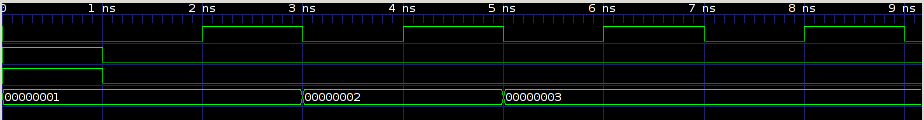
\includegraphics[width=10cm]{capture-chrono-bitcompteur.png}
    \end{center}
  \end{block}

  \begin{block}{Synthèse}
    \textit{Xilinx XST} synthétise une netlist avec des propriétés
    satisfaisantes :

    \begin{itemize}
    \item Deux additionneurs 32 bits.
    \item Un registre 1 bit.
    \end{itemize}
  \end{block}
\end{frame}

\end{document}
